%
% Main document
% ===========================================================================
% This is part of the document "Project documentation template".
% Authors: brd3, kaa1
%

%---------------------------------------------------------------------------
\documentclass{bfh_template}
\usepackage[titletoc]{appendix}
\usepackage{tikz}
\usetikzlibrary{arrows,shadows}
\usepackage{pgf-umlsd}
\usepackage{listings}
\usepackage{listings}
\usepackage{color}
\definecolor{lightgray}{rgb}{.9,.9,.9}
\definecolor{darkgray}{rgb}{.4,.4,.4}
% Documentation https://www.sharelatex.com/learn/Code_listing
% From https://gist.githubusercontent.com/Geruhn/3d21f60a869457373d84/raw/88f5e81e6eb00e7aa47be8aaf1061682f053eae9/lstset_js.tex

\definecolor{purple}{rgb}{0.65, 0.12, 0.82}
\lstdefinelanguage{JavaScript}{
  keywords={break, case, catch, continue, debugger, default, delete, do, else, false, finally, for, function, if, in, instanceof, new, null, return, switch, this, throw, true, try, typeof, var, void, while, with},
  morecomment=[l]{//},
  morecomment=[s]{/*}{*/},
  morestring=[b]',
  morestring=[b]",
  ndkeywords={class, export, boolean, throw, implements, import, this},
  keywordstyle=\color{blue}\bfseries,
  ndkeywordstyle=\color{darkgray}\bfseries,
  identifierstyle=\color{black},
  commentstyle=\color{purple}\ttfamily,
  stringstyle=\color{red}\ttfamily,
  sensitive=true
}

\lstset{
   language=JavaScript,
   backgroundcolor=\color{white},
   extendedchars=true,
   basicstyle=\footnotesize\ttfamily,
   showstringspaces=false,
   showspaces=false,
   numbers=left,
   numberstyle=\footnotesize,
   numbersep=9pt,
   tabsize=2,
   breaklines=true,
   showtabs=false,
   captionpos=b
}


%---------------------------------------------------------------------------
%  Read title, version number and date of the paper from the file:
%  title_version_def.tex
\providecommand{\titel}{Metropolitan-Sensor/Aktor-Netze unter Einsatz von LoRa und anderen Techniken}					%  Hier den Titel des Berichts/Thesis eingeben
\providecommand{\versionnumber}{1.0}			%  Hier die aktuelle Versionsnummer eingeben
\providecommand{\versiondate}{25.06.2016}		%  Hier das Datum der aktuellen Version eingeben


%---------------------------------------------------------------------------
\begin{document}                        % Start Document


%---------------------------------------------------------------------------
% Title Page and Abstract
%---------------------------------------------------------------------------
%\include{lead/titelseite_ohne_bild}	% activate for Titelseite ohne Bild
%
% Project documentation template
% ===========================================================================
% This is part of the document "Project documentation template".
% Authors: brd3, kaa1
%

\begin{titlepage}


% BFH-Logo absolute placed at (28,12) on A4 and picture (16:9 or 15cm x 8.5cm)
% Actually not a realy satisfactory solution but working.
%---------------------------------------------------------------------------
\setlength{\unitlength}{1mm}
\begin{textblock}{20}[0,0](28,12)
	
\includegraphics[scale=1.0]{pictures/BFH_Logo_B.png}
\end{textblock}

\begin{textblock}{154}(28,48)
	\begin{picture}(150,2)
		\put(0,0){\color{bfhgrey}\rule{150mm}{2mm}}
	\end{picture}
\end{textblock}

\begin{textblock}{154}[0,0](28,50)
	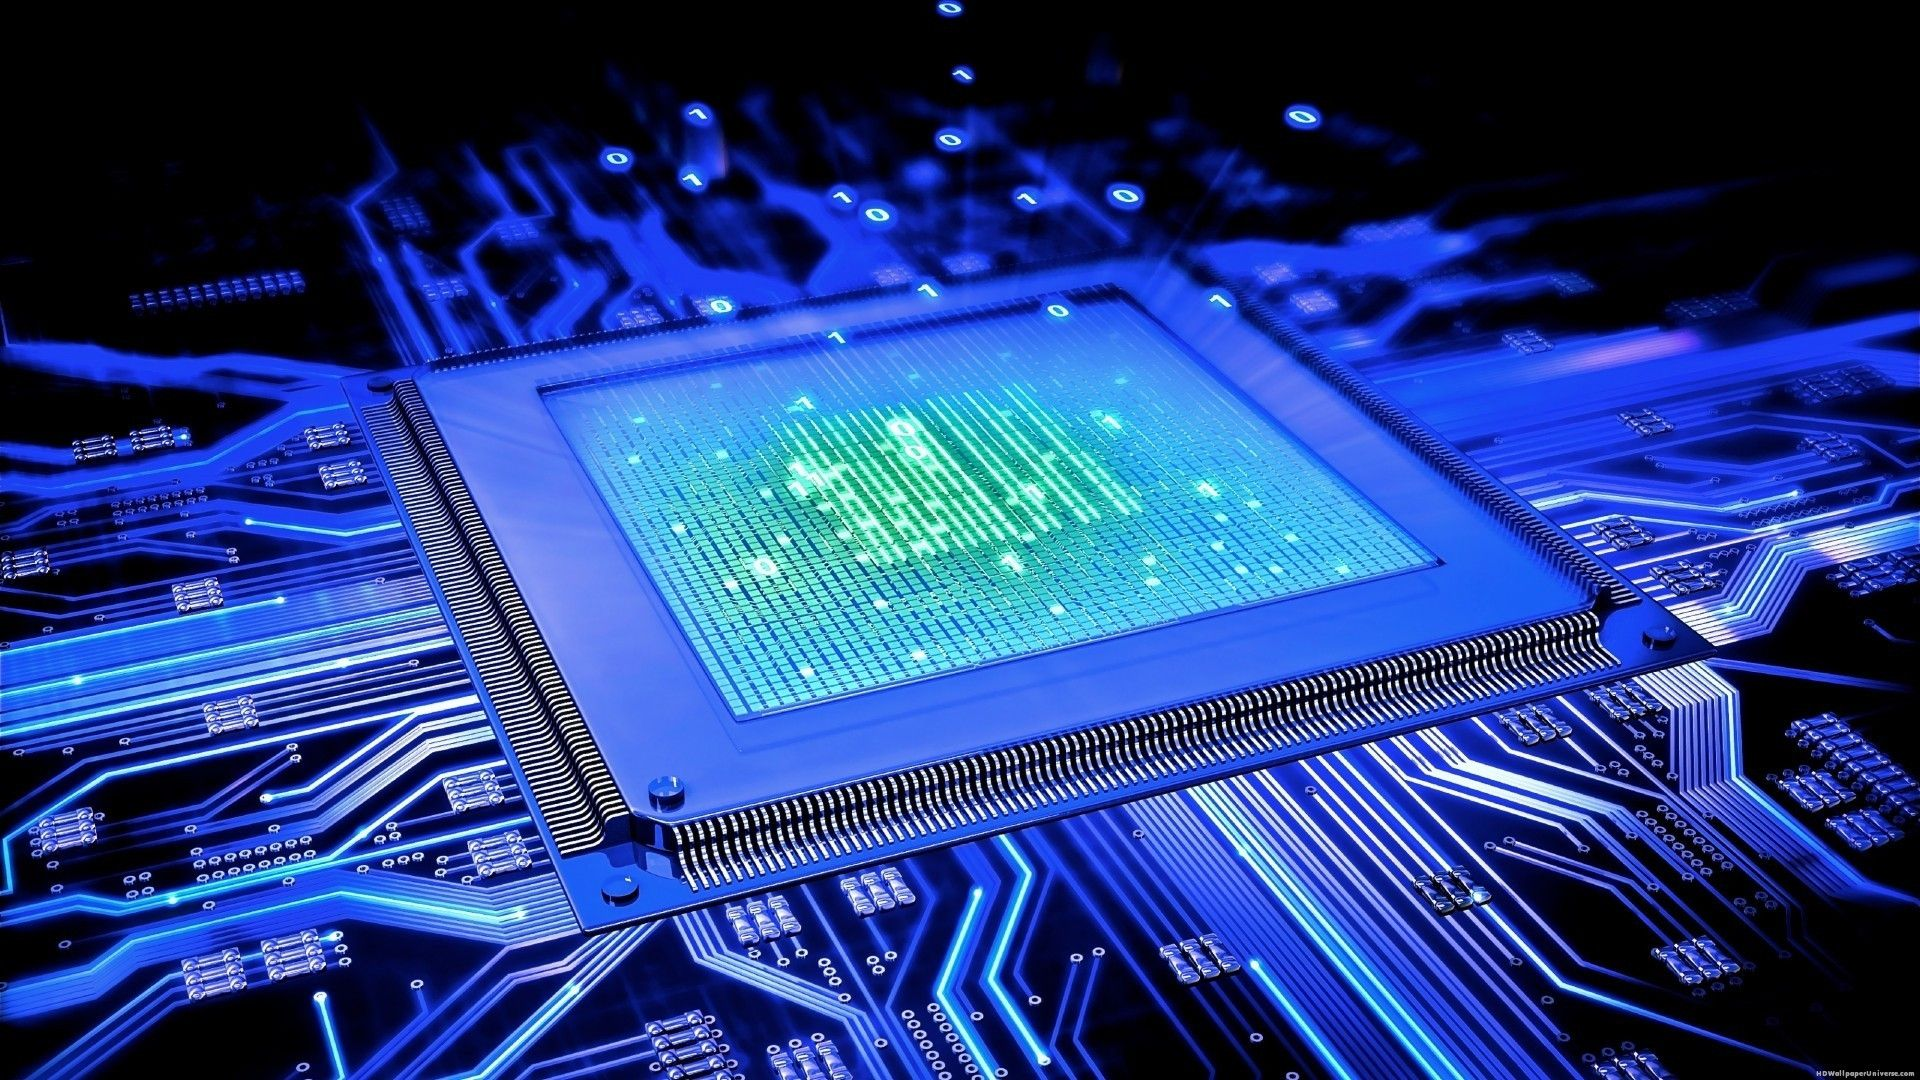
\includegraphics[height=85mm,width=150mm]{pictures/cs.jpg}
%\includegraphics[width=150mm]{pictures/network-782707_1280.png}			% Titelbild definieren
%1.764705882
\end{textblock}

\begin{textblock}{154}(28,135)
	\begin{picture}(150,2)
		\put(0,0){\color{bfhgrey}\rule{150mm}{2mm}}
	\end{picture}
\end{textblock}
\color{black}

% Institution / Titel / Untertitel / Autoren / Experten:
%---------------------------------------------------------------------------
\begin{flushleft}

\vspace*{115mm}

\fontsize{26pt}{28pt}\selectfont
\titel 								\\ % Titel aus der Datei lead/titel.tex lesen
\vspace{2mm}

% \fontsize{16pt}{20pt}\selectfont\vspace{0.3em}
% Subtitle 	\\ % Untertitel eingeben
% \vspace{5mm}

\fontsize{10pt}{12pt}\selectfont
\textbf{Projekt 2} \\ % eingeben
\vspace{3mm}

% Abstract (eingeben):
%---------------------------------------------------------------------------
%\begin{textblock}{150}(28,190)
%\fontsize{10pt}{12pt}\selectfont
%[Kurztext (Abstract) einfügen, falls gewünscht] \\
%Dieses Dokument dient als Vorlage für die Erstellung von Berichten nach den Richtlinien der BFH. Die Vorlage ist %in \LaTeX{} erstellt und unterstützt das automatische Erstellen von diversen Verzeichnissen, Literaturangaben, %Indexierung und Glossaren. Dieser kleine Text ist eine Zusammenfassung über das vorliegenden Dokument mit einer %Länge von 4 bis max. 8 Zeilen. \\
%Das Titelbild kann in den Zeilen 157/158 der Datei template.tex ein- oder ausgeschaltet werden.
%\end{textblock}

\begin{textblock}{150}(28,225)
\fontsize{10pt}{17pt}\selectfont
\begin{tabbing}
xxxxxxxxxxxxxxx\=xxxxxxxxxxxxxxxxxxxxxxxxxxxxxxxxxxxxxxxxxxxxxxx \kill
\\
\\
Studiengang:	\> Bachelor of Science Informatik	\\	% Namen eingeben
Autor:			\> Simon Wittwer, Marc Zimmermann	\\	% Namen eingeben
Betreuer:		\> Dr.~Andreas Danuser				\\	% Namen eingeben
% Experte:		\> Don Mutex						\\	% Namen eingeben
Datum:			\> \versiondate						\\	% aus Datei lead/versions.tex lesen
\end{tabbing}

\end{textblock}
\end{flushleft}

\begin{textblock}{150}(28,280)
\noindent
\color{bfhgrey}\fontsize{9pt}{10pt}\selectfont
Berner Fachhochschule | Haute école spécialisée bernoise | Bern University of Applied Sciences
\color{black}\selectfont
\end{textblock}


\end{titlepage}

%
% ===========================================================================
% EOF
%
				% activate for Titelseite mit Bild
% Versionenkontrolle :
% -----------------------------------------------

\null
\vfill

\begin{Large}
Versionen
\end{Large}

\fontsize{10pt}{18pt}\selectfont
\begin{tabbing}
xxxxxxxxxxx\=xxxxxxxxxxxxxxx\=xxxxxxxxxxxxxx\=xxxxxxxxxxxxxxxxxxxxxxxxxxxxxxxxxxxxxxxxxxxxxxx \kill
Version	\> Datum	\> Status		\> Bemerkungen		\\
0.1	\> 22.04.2016	\> Entwurf		\> Latex-Dokument eingerichtet	\\
0.1.1\> 23.04.2016	\> Entwurf		\> Kapitelstruktur erstellt \\
0.2	\> 12.06.2016	\> Entwurf		\> Anforderungen \\
0.3	\> 11.06.2016	\> Entwurf		\> Kapitel Einleitung \\
0.4	\> 18.06.2016	\> Entwurf		\> Kapitel Anwendungsfälle und Anforderungen \\
0.5	\> 20.06.2016	\> Entwurf		\> Kapitel Rahmenbedingungen \\
0.6	\> 20.06.2016	\> Entwurf		\> Kapitel Use Case Tresh \\
0.7	\> 23.06.2016	\> Entwurf		\> Kapitel Drahtlose Datenübertragung \\
0.8	\> 24.06.2016	\> Entwurf		\> Kapitel Prototyp, Resultate, Anhang \\
0.9	\> 25.06.2016	\> Entwurf		\> Management Summary, Fazit und Korrektur lesen \\
1.0	\> 25.06.2016	\> Final		\> Finale Version \\
\end{tabbing}


\cleardoubleemptypage
%\setcounter{page}{1}

\cleardoublepage
\phantomsection
% % \chapter*{Summary}\label{summary}
% \addcontentsline{toc}{chapter}{Summary}

\begin{abstract}
{\huge Management Summary\par} % parens are here to define the scope of \huge and \par
% \lipsum[1]
Diese Arbeit befasst sich im Rahmen des Projekt 2 mit verschiedenen Aspekten von \gls{iot}. Einerseits wird versucht mit der Auseinandersetzung von möglichen Use-Cases über verschiedene Branchen hinweg, ein Gefühl für das Marktpotential und die Herausforderungen von \gls{iot} zu entwickeln und daraus gleichzeitig wichtige Anforderungen an \gls{iotk} abzuleiten. Andererseits wird mit der Gegebüberstellung der wichtigsten Funktechnologien und deren Vor- und Nachteilen eine Übersicht verschafft und die auf Spreizbandmodulation basierende Technologie \gls{lora} vertieft betrachtet.\\
Um die verschiedenen Aspekte schliesslich zu kombinieren, wird der konkrete Use-Case \glqq{}Tresh\grqq{} vorgestellt und dessen Implementation und die gewonnenen Erfahrungen anhand eines Prototypen aufgezeigt.
\end{abstract}

% \chapter*{Summary}\label{summary}
% \addcontentsline{toc}{chapter}{Summary}

\begin{abstract}
{\huge Management Summary\par} % parens are here to define the scope of \huge and \par
% \lipsum[1]
Diese Arbeit befasst sich im Rahmen des Projekt 2 mit verschiedenen Aspekten von \gls{iot}. Einerseits wird versucht mit der Auseinandersetzung von möglichen Use-Cases über verschiedene Branchen hinweg, ein Gefühl für das Marktpotential und die Herausforderungen von \gls{iot} zu entwickeln und daraus gleichzeitig wichtige Anforderungen an \gls{iotk} abzuleiten. Andererseits wird mit der Gegebüberstellung der wichtigsten Funktechnologien und deren Vor- und Nachteilen eine Übersicht verschafft und die auf Spreizbandmodulation basierende Technologie \gls{lora} vertieft betrachtet.\\
Um die verschiedenen Aspekte schliesslich zu kombinieren, wird der konkrete Use-Case \glqq{}Tresh\grqq{} vorgestellt und dessen Implementation und die gewonnenen Erfahrungen anhand eines Prototypen aufgezeigt.
\end{abstract}

\cleardoubleemptypage

%---------------------------------------------------------------------------
% Table of contents
%---------------------------------------------------------------------------
\tableofcontents

%---------------------------------------------------------------------------
% Main part
%---------------------------------------------------------------------------
\cleardoublepage
\pagenumbering{arabic}
\chapter{Einleitung}

\acrfull{iot} hat laut Gartner gerade den Höhepunkt des Hypes erreicht. Der Begriff ist in aller Munde und jeder kennt es. Doch wo sind solche "Things" tatsächlich bereits anzutreffen? Diese Arbeit behandelt das Thema "Metropolitan-Sensor/Aktor-Netze unter Einsatz von LoRa und anderen Techniken". Sie sucht nach Anwendungsfällen wo solche Things, auch \gls{iotk} genannt, im urbanen Umfeld sinnvoll eingesetzt werden können.\\
Ein \gls{iotk} ist ein Mikrocontroller, welcher Sensoren und Aktoren verwaltet. Die Sensordaten sendet er über eine Verbindung zu einem Gateway, welches die Daten wiederum an einen Server oder in die Cloud leitet. Umgekehrt können vom Server oder von der Cloud Befehle über das Gateway an den Controller geschickt werden. Der Controller steuert damit die Aktoren. Aus solchen \gls{iotk} und  Gateways entsteht schliesslich ein Sensor-Aktor-Netz. Für dieses Netz spielt die Verbindung zwischen den IoT-Knoten und den Gateways eine sehr wichtige Rolle. Sie definiert Faktoren wie Distanz, Bandbreite und Energieverbrauch. Diese Faktoren sind für einen \gls{iotk} von entscheidender Bedeutung da sie direkten Einfluss auf dessen Lebensdauer und seine Kosten haben. Ebenso beschränkt es die Grösse des Netzes, je nachdem welche Reichweite mit der Verbindung möglich ist. Da die \gls{iotk} oft an Orten eingerichtet werden wo weder eine Netzwerk-Anbindung noch Energieversorgung verfügbar ist, muss der Sensor möglichst autark sein. Das bedingt eine drahtlose Verbindung zwischen der Knoten und der Gateways. Aus diesem Grund behandelt die Arbeit unter anderem verschiedene Funk-Standards, welche zurzeit existieren und in den Frequenzen eines \gls{ism}es sind, damit keine Lizenzen die Kosten der \gls{iotk} in die Höhe treiben. LoRa, eine Funkmodulationstechnik hat seine Stärken genau in den Faktoren Distanz und Energieverbrauch, weshalb sie ideal für solche Verbindungen geeignet scheint. Aus diesem Grund implementiert diese Arbeit ein Proof-of-concept mit diesem Standard. 
\chapter{Anwendungsfälle für IoT}

\chapter{Rahmenbedingungen für \gls{iot}} \label{Rahmenbedingungen für iot}
Die Use Cases aus den verschiedensten Branchen zeigen: in praktisch jeder Lebenssituation können Dinge automatisiert oder verbessert werden. So manchen Prozess, welchen wir heutzutage regelmässig wiederholen, kann automatisiert oder zumindest zeitlich optimiert werden, so dass er nur ausgeführt wird, wenn er wirklich nötig ist. Viele der beschriebenen Use Cases sind von mehreren Faktoren Abhängig. Der in Smart Home beschriebene Wecker benötigt beispielsweise folgende Sensoren und Aktoren:
\begin{itemize}  
  \item Zeit-Sensor (Real-Time Clock)
  \item Wetter-Sensor (Licht-Sensor vor dem Fenster)
  \item Schlafphasen-Sensor (Smartwatch)
  \item Aufsteh-Sensor (Bodenplatten-Sensoren oder Smartwatch)
  \item Storen-Aktor (Elektrisch gesteuerte Storen)
  \item Licht-Aktor (Smarte LEDs)
  \item Musik-Aktor (Smarte Stereoanlage)
\end{itemize}
Dieser Wecker funktioniert erst, wenn der Wecker alle diese Sensoren auslesen kann und die Aktoren steuern kann. Natürlich könnte ein Wecker konstruiert werden, welcher all diese Informationen für sich erfasst und so autonom funktioniert. Es existieren mittlerweile auch bereits alle Sensoren und Aktoren für sich. Allerdings wäre ein solch intelligenter Wecker als Komplettprodukt viel zu teuer und nicht erweiterbar. Deshalb ist es viel sinnvoller, wenn Sensoren ihre Daten an eine \gls{iotp} senden, welche die Sensordaten über standardisierte Schnittstellen empfängt und danach für Aktoren wieder über Schnittstellen bereitstellt. Erst mit einer solchen Plattform kann \gls{iot} sein Potential ausschöpfen. Durch das Teilen von Informationen können Sensoren und Aktoren voneinander profitieren.
Somit muss nicht jedes System seine eigenen Sensoren und Aktoren zur Verfügung stellen. Redundanzen können verhindert werden. Dies ermöglicht, dass komplexe Systeme rasch und effizient entstehen können.  

\section{\gls{iotk}}
Heutzutage existieren bereits viele Sensoren und Aktoren. Beispielsweise haben die meisten aktuellen Smartphones Sensoren für Helligkeit, Temperatur, Beschleunigung Neigung, Position, Feuchtigkeit und Näherung. Leider befinden sich Smartphones einem grossen Teil der Zeit in Hand- oder Hosentaschen, weshalb die Sensoren für die meisten Anwedungsfälle keine sinnvollen Daten messen. Weiter verwenden  Smartphones die Kostenpflichtigen 2/3/4G-Netzwerke. Dies ist finanziell nicht interessant und energetisch nicht sinnvoll, da diese Netzwerke nicht für Niedrigst-Energie-Geräte entwickelt wurden. Aus diesen Gründen eignen sich Smartphones eher schlecht als \gls{iotk}. Damit ein \gls{iotk} sinnvoll eingesetzt werden kann, sollte er nur die nötigsten Sensoren haben und diese müssen sinnvoll positioniert sein, damit sie die Daten für den Use Case optimal ermitteln können. Statt also auf ein mit Sensoren vollgepacktes Gerät, wie ein Smartphone, aufzusetzen, macht es mehr Sinn neue Sensor-Knoten zu bauen, welche speziell auf einen Use Case abgestimmt sind.

\section{\gls{iotp}}
Wie bereits erwähnt brauchen die \gls{iotk} eine zentrale Stelle, welche die Sensordaten entgegennimmt und bei bedarf speichern, aggregieren oder manipulieren kann. Das Unterenehmen Appmodule entwickelt unter der Leitung von Andreas Danuser eine solche Plattform. 
\subsection{SIOT.net}
SIOT.net bietet Schnittstellen via MQTT, WebSocket sowie REST um Sensor-Daten entgegenzunehmen. Zugleich bietet Sie die Möglichkeit mit Node-Red, die Daten zu aggregieren und Events auszulösen oder Aktoren zu steuern. Weiter bietet sie eine Art Dashboard in welcher die Sensorwerte präsentiert werden können.

\section{\gls{iotg}}
Zur Verbindung der \gls{iotk} und der \gls{iotp} wird schliesslich ein Gateway benötigt. Dieses empfängt die Funkdaten verschiedener Knoten und sendet sie an die Plattform mit zusätzlichen Informationen wie Beispielsweise der Sensor-ID oder der Empfangsqualität des Empfangenen Pakets. Das Gateway ist somit einerseits ein Übersetzer von \gls{iot}-Kommunikation zu klassischer Netzwerk-Kommunikation, andererseits hat es auch noch eine Sensor-Funktion, da es den Zustand der Kommunikation und des \gls{iot}-Netzes an die Plattform meldet. 

\begin{figure}[H]
    \centering
        \includegraphics[width=1.0\textwidth]{pictures/IoT_Conditions.png}
    \caption{IoT Module}
    \label{fig:IoT Module}
\end{figure}


\chapter{Anforderungen an \gls{iotk}}

Durch das Analysieren von Anwendungsfällen im vorherigen Kapitel, haben sich wichtige Anforderungen an \gls{iotk} herauskristallisiert. Nachfolgend werden diese genauer beschrieben.

\section{Reichweite}

Je nach Anwendungsfall gibt es unterschiedliche Anforderungen an die Reichweite eines \gls{iotk}. Die flexibelste Art Daten zu Senden und Empfangen ist über eine drahtlose Funkverbindung. Bei kurzen Distanzen und vorhandener Energieversorgung genügen oft konventionelle Technologien wie \gls{wifi} oder \gls{bluetooth}. Sobald aber die Distanzen zwischen den \gls{iotk} grösser werden und zusätzlich noch Hindernisse wie Gebäude oder Hügel überwunden werden müssen, werden andere Technologien benötigt. Die Funkmodulationstechnik \gls{lora} erlaubt das Übertragen von Daten über mehrere Kilometer, doch nicht ohne dabei einen Kompromiss einzugehen. Grundsätzlich gilt: Je tiefer die Übertragungsfrequenz desto grösser ist die Reichweite und umso kleiner ist der Datendurchsatz. Das heisst bei \gls{lora} kann eine Vergrösserung der Reichweite auf Kosten des Datendurchsatzes erreicht werden. Die physikalischen Gesetze zwingen zu einem Abwägen zwischen Reichweite und Datendurchsatz bei der Wahl der geeigneten Funk-Technologie für ein Sensor/Aktor Netzwerk. Diese Tatsache hat noch weitere Implikationen auf andere Anforderungen wie Verwaltbarkeit und Datendurchsatz.

\section{Datendurchsatz}

Je nach dem wie viele Daten in einem Sensor/Aktor Netzwerk anfallen, wird ein unterschiedlicher Datendurchsatz benötigt. Wie im oberen Abschnitt beschrieben beeinflusst der Datendurchsatz die mögliche Reichweite und somit die Wahl der geeigneten Technologien. Über eine \gls{wifi} 802.11n Verbindung können bis zu 300Mbs übertragen werden, d.h. Bild- , Audio- und Videodaten können ohne Probleme in kurzer Zeit übertragen werden. Sogar das Streaming von hochauflösenden Videodaten ist möglich. Im Gegensatz dazu ist es in einem \gls{lora}-Netzwerk äusserst ineffizient Bilddaten zu übertragen und undenkbar Videostreaming zu betreiben, denn die maximale Datenrate von \gls{lora} (Mode 10) beträgt 38.4kbps \autocite[2]{lora:FAQ}.\\
Ein weiterer Faktor der den Datendurchsatz beeinflusst ist die Anzahl Teilnehmer in einem Netz die gleichzeitig Daten versenden. Wenn nur ein einzelner Knoten Daten versendet, kann er die volle Datenrate ausnutzen. Mit jedem weiteren Teilnehmer der dazu kommt, muss die Datenrate geteilt werden.\\
Bei der Wahl eines \gls{iotk} ist der Datendurchsatz also ein wichtiges Entscheidungskriterium. Je nach Anwendungsfall muss zischen Datendurchsatz, Reichweite und Anzahl Teilnehmer im Netzwerk abgewogen werden.

\section{Zuverlässigkeit}

Eine weitere wichtige Anforderung an einen \gls{iotk} ist seine Zuverlässigkeit. Grundsätzlich ist hiermit der Determinismus des Systems gemeint, also dass sich das System immer gleich verhält und dieses Verhalten klar bestimmt ist. Konkret müssen folgende Kriterien eines \gls{iotk} Zuverlässig sein:
\begin{itemize}  
  \item Messresultate der Sensoren
  \item Funktion der Aktoren
  \item Übertragung der Daten
  \item Übertragungszeit im Netzwerk (Jitter)
  \item Entladekurve der Energiespeicher
\end{itemize}

Mit einer hohen Zuverlässigkeit kann ein System optimal operieren, insbesondere über einen längeren Zeitraum. Der Wartungsaufwand kann minimiert und genauer geplant werden. Da durch den deterministischen Charakter einige Parameter des Systems berechenbar werden, lassen sich daraus leicht einige Annahmen ableiten.

\section{Sicherheit}

Die Frage nach der Sicherheit eines Systems ist ein Dauerbrenner in der Informationstechnologie. So auch im \acrshort{iot}-Sektor. Je nach dem wie sensibel die Daten sind, die mit einem \gls{iotk} gemessen und übertragen werden, müssen andere Sicherheitsmassnahmen getroffen werden. Die \gls{iotk} sollten eine eingebaute Hardwarebeschleunigung für kryptographische Operationen unterstützten, wie z.B. AES-Beschleunigung. Für hochsensible Daten ist die Möglichkeit der End-zu-End Verschlüsselung vom Sensor bis zum Endnutzer nötig, was die Komplexität des Systems massiv erhöhen kann. Auch hier muss anhand der Anforderungen der Anwendung zwischen mehr Sicherheit oder mehr Akkulaufzeit (da keine zusätzlichen Chips für die Hardwarebeschleunigung benötigt werden) und Flexibilität abgewogen werden.

\section{Topologie}

Je nach Anwendungsgebiet und verwendeter Technologie sind unterschiedliche Netzwerk Topologien sinvoll. Die einfachste Topologie ist eine Punkt-zu-Punkt Verbindung. Dabei sind genau zwei Knoten miteinander verbunden. Während diese Topologie sehr einfach ist, ist sie gleichzeitig sehr eingeschränkt, da nur zwei Teilnehmer miteinander kommunizieren können. In einem Mesh Netzwerk leiten die Endknoten Daten von anderen Knoten weiter, um die Reichweite und die Anzahl Teilnehmer der Netzwerk-Zelle zu erhöhen. Dafür erhöht sich aber auch die Komplexität und Netzwerkkapazität. In einem Stern Netzwerk sind mehrere Teilnehmer mit einem zentralen \gls{iotg} verbunden. Die Teilnehmer können über dieses \gls{iotg} mit den anderen Teilnehmern kommunizieren. So kann viel Logik von den Knoten weg in das \gls{iotg} verschoben werden, was im Falle der \glspl{iotk} ein einfacheres Design erlaubt. Da es mehr \gls{iotk} als \glspl{iotg} gibt, hat dies auch einen Kosten-Nutzen.

\section{Energieverbrauch}

Ein kritischer Faktor für jeden \gls{iotk} ist der Energieverbrauch. Dieser ist von verschiedenen Faktoren wie Standort, Art und Anzahl Sensoren und Aktoren, Messintervallen und Operationen, verwendeter Hardwarekomponenten und verfügbarem Platz abhänging.\\
Ein idealer Standort eines Knotens hätte eine bereits vorhandene, stetige Energiequelle. Doch dies ist in der Praxis selten der Fall, da die Knoten oft an Orten mit keiner oder nur begrenzter Energieversorgung eingesetzt werden. Daher wird Platz für einen Energiespeicher benötigt. Optimal ist es, am Standort Energie zu gewinnen, beispielsweise mit Solarzellen. Der Energiespeicher ist somit ein Puffer, da die Gewinnung nicht konstant ist. \gls{iotk} werden oft in bestehende Systeme integriert, weshalb die Platzverhältnisse stark begrenzt sind. Diese knappen Verhältnisse schränken die Grösse des Energiespeichers und auch die Möglichkeiten der Energiegewinnung ein. Damit wird jedes Miliampere zu einem kostbaren Gut und ein haushälterischer Umgang damit verlängert die Lebensdauer und vermindert Wartungseinsätze.\\
Ein effizientes Energiemanagement kann mit dem Einsatz von auf den Anwendungsfall reduzierter Hardware, die es erlaubt in einen Energiesparmodus zu wechseln und dafür optimierter Software sichergestellt werden.

\subsection{Intelligente Messungen}

Um die gewünschten Informationen für die Anwendung mithilfe eines \glspl{iotk} zu ermitteln, sind auf den Anwendungsfall zugeschnittene, intelligente Messungen sehr wertvoll. Zwar könnte man einen Sensor so oft wie möglich auslesen und alle diese Werte über das Netzwerk in die Cloud speichern. Doch meistens ist dies gar nicht notwendig. Es erhöht nur unnötig den Energieverbrauch und die Auslastung des Netzwerks.\\
Je nach Anwendungsfall sind unterschiedliche Messarten sinnvoll. Diese können grundsätzlich in zwei Klassen aufgeteilt werden: Messungen können entweder durch einen Trigger oder zu definierten Zeitpunkten ausgelöst werden. Das ereignisbasierte Auslösen durch einen Trigger ist zum Beispiel beim Herausfinden ob eine Tür offen oder geschlossen ist sinnvoll. Nur die Zustandsänderung ist von Interesse, nicht aber eine dauernde Überwachung. Bei einer Anwendung wo es nicht möglich ist einen zuverlässiges Ereignis zu triggern, muss mit zeitzyklischen Messungen gearbeitet werden. Dabei muss bei der Bestimmung der Messintervalle zwischen Genauigkeit und Energieverbrauch abgewogen werden. Zusätzlich können Knoten während Zeiten, wo keine Messungen benötigt werden in den Energiesparmodus wechseln oder ganz abgeschaltet werden. Ein Beispiel dafür sind Alarmanlagen, sie müssen nur aktiv sein wenn kein Personal anwesend ist.

\section{Verwaltbarkeit}

Wenn einmal ein Netz von \gls{iotk} aufgebaut ist, stellt sich schnell einmal die Frage wie Änderungen an alle Knoten propagiert werden können. Je nach Topologie, Datendurchsatz und Intelligenz der Knoten bieten sich unterschiedliche Möglichkeiten an. Diese lassen sich in folgende vier Stufen aufteilen:

\begin{enumerate}
  \item Nur lokaler Zugriff
  \item Remote Reset des \gls{iotk}
  \item Remote Konfiguration einzelner Parameter des \gls{iotk}
  \item Remote \acrfull{ota}-Update 
\end{enumerate}

\section{Benutzerfreundlichkeit}

Je nachdem von welcher Zielgruppe schlussendlich die \glspl{iotk} verwendet werden, verändern sich auch die Anforderungen an die Benutzerfreundlichkeit der Knoten. Angenommen ein Parkhaus hat alle Parkfelder komplett neu mit Parksensoren ausgestattet. Der Abwart des Parkhauses ist neu für die Wartung aller Parksensoren verantwortlich. Seine Hauptaufgabe ist eine regelmässige Funktionskontrolle der Sensoren. Das Softwareunternehmen, welches das \acrshort{iot}-System entwickelt und integriert hat, ist verpflichtet das System weiter zu verbessern und will daher möglichst viel Kontrolle über die \gls{iotk} haben. Darum will das Unternehmen die Software möglichst Remote verwalten und aktualisieren können.
Die im vorderen Abschnitt erwähnten vier Stufen könnten wie folgt aussehen:

\textbf{Funktionskontrolle der Sensoren}
\begin{enumerate}  
  \item Der Abwart muss bei jedem \gls{iotk} vorbeigehen und eine Funktionskontrolle durchführen.
  \item Der Abwart kann zumindest versuchen einen defekten \gls{iotk} zuerst über eine Smartphone App zurückzusetzen, bevor er vorbeigehen muss.
  \item Der Abwart kann defekte \gls{iotk} über die Smartphone App identifizieren und gezielt reparieren.
  \item Der Abwart kann ein Zeitfenster definieren in welchem die Sensoren oder eine Sensorgruppe aktualisiert werden darf.
\end{enumerate}

\textbf{Software aktualisieren}
\begin{enumerate}  
  \item Das Untenehmen muss einen Mitarbeiter vorbeischicken der bei jedem \gls{iotk} vorbeigeht und von Hand flasht oder den Abwart instruieren.
  \item Wie Stufe 1.
  \item Die Entwickler können grosse Teile der Funktionalität ändern, wenn sie möglichst viel Logik in die \glspl{iotg} verlagern und auf den \gls{iotk} viele flexible Parameter definieren.
  \item Die Entwickler können die gesamte Software Remote ändern.
\end{enumerate}

\section{Kosten}

Ein entscheidender Faktor sind schlussendlich auch die Kosten. Der erste wichtige Kostenfaktor sind die Anschaffungskosten. Je tiefer der Preis pro \gls{iotk}, desto günstiger wird das Gesamtsystem. Wenn die Hardwarekomponenten genau auf den jeweiligen Anwendungsfall reduziert werden, können die Produktionskosten minimiert werden, was sich auf die Anschaffungskosten auswirkt. Dies hat auch meist auch positive Auswirkungen auf die Energieeffizienz der \gls{iotk}.\\
Ein weiterer Kostenfaktor sind die Wartungskosten. Umso länger ein \gls{iotk} zuverlässig läuft, desto weniger Kosten für die Wartung fallen an. Das heisst es können Personalkosten gespart werden, da sich niemand um defekte Knoten kümmern oder Akkumulatoren austauschen muss. Je länger und zuverlässiger ein \gls{iotk} ununterbrochen seinen Dienst verrichtet, desto weniger Betriebskosten fallen an. Ein zusätzlicher Kostenfaktor für den Betrieb ist die Wahl des Frequenzbandes. Wird zum Beispiel \gls{lora} eingesetzt, fallen gar keine Kosten für die Nutzung des Frequenzbandes an, da \gls{lora} ein \gls{ism} nutzt. Wird ein kostenpflichtiges Frequenzband eingesetzt, kann dies einen signifikanten Anteil an den Betriebskosten ausmachen. Ein letzter wichtiger Kostenfaktor ist die Zuverlässigkeit eines \gls{iotk} und ein möglichst geringer Verschleiss.

\chapter{Drahtlose Datenübertragung}

Der Bedarf an drahtlosen Technologien im industriellen sowie im privaten Umfeld steigt immer mehr. Die Schlüsselfaktoren, die hinter den Anforderungen für drahtlose Technologien stehen, sind zum einen die Fernsteuerung, damit verbunden die Mobilität und Flexibilität, zum anderen die verschleissfreie Übertragung von Daten. Beispielsweise können drahtlose Sensoren und Aktoren, die auf beweglichen Teilen von Maschinen positioniert werden, von Vorteil für drahtlose Systeme sein. Jede Anwendung hat unterschiedliche Anforderungen. Es gibt kein einzelnes drahtloses System, das alle Anforderungen gleichzeitig erfüllen kann.\\
Im Rahmen dieser Arbeit wurden mehrere Funktechnologien die im \acrshort{iot}-Umfeld in Frage kommen angeschaut und deren Vor- und Nachteile aufgezeigt, die nachfolgend beschrieben werden.

\section{BLE}

\section{BLE}
\chapter{Der Use Case Tresh}

\section{Entwicklung des Use Case}\label{chapter:devOfUseCase}
Durch den ersten Teil der Arbeit, der Analyse von Rahmenbedingungen, Anforderungen und technischen Möglichkeiten für Funktechnologien von \gls{iotk}, hat sich gezeigt, dass \gls{lora} in praktisch allen Bereichen ein optimales Verhältnis zu allen Anforderungen hat. Nun ist als zweiter Teil der Arbeit das Ziel, anhand eines praktischen Use Cases diese Technologie effektiv einzusetzen und dadurch erste Erfahrungen damit zu sammeln. Mit der \gls{pshmthd} soll nun ein Bedürfnis gefunden werden, welches zu der \gls{lora}-Technologie passt. Dabei kommen als erstes natürlich die Use Cases aus dem Kapitel \ref{Anwendungsfälle für IoT} zur Evaluation. Es stellte sich aber heraus, dass die meisten Use Cases den Rahmen des Projekt 2 sprengen würden. Das grösste Problem vieler Use Cases sind die verschiedenen Abhängigkeiten. So wie in den Rahmenbedingungen in Kapitel \ref{Rahmenbedingungen für iot} beschrieben, hat ein intelligentes \gls{iot}-System schnell einmal Abhängigkeiten von mehreren Sensoren und Aktoren. Die Sensoren und Aktoren haben wiederum eine Menge Schnittstellen, welche zu verbinden sind. Wir mussten feststellen, dass unser Brainstorming noch nicht zum Erfolg führte. Doch wie so oft kommen die Ideen nicht beim Brainstorming, sondern dann wenn man nicht damit rechnet: in unserem Fall war es Frust über einen vollen Mülleimer. Dies brachte den Lichtblitz: Der Füllstand von Mülleimern muss überwacht werden, damit die Eimer früh genug entleert werden können und Sauereien verhindert werden können.

\begin{figure}[H]
     \centering
        \includegraphics[width=1.0\textwidth]{pictures/TRESH_Idea.png}
    \caption{Entwicklung des TRESH: vom Wägen über Lichtschranken zur Ultraschall-Distanzmessung}
    \label{fig:TRESH Idee}
\end{figure}

Das Überwachen des Füllstandes kann ein einfacher \gls{iotk} übernehmen. Es entstehen dabei keinen Abhängigkeiten und es müssen nicht mehrere Sensoren kombiniert werden. Ein Idealer Use Case für dieses Projekt. Als erstes musste eine sinnvolle Messmethode für den Füllstand gefunden werden. Die erste Idee: eine Waage. Diese misst jedoch das Gewicht des Mülls anstelle des Volumens. Lichtschranken könnten in verschiedenen Höhen des Eimers positioniert werden. Wenn die Schranken unterbrochen werden hat der Müll den Füllstand mindestens auf die Höhe dieser Schranke erreicht. Diese Messmethode scheint zuverlässig, benötigt aber ein komplexes Design des Mülleimers. Ausserdem benötigt diese Methode transparente Müllsäcke, was eher selten ist. Zudem sind die Lichtschranken in Gefahr durch den Müll verschmutzt zu werden und daher anfällig für Fehlmessungen. Besser wäre es also von der Decke aus zu messen. So ist der Müllsack nicht gestört und das Risiko, dass der Sensor durch Müll verschmutzt wird ist auch viel kleiner. Für Distanzmessungen wäre Laser eine Möglichkeit. Der dünne Laserstrahl misst aber nur einen Punkt, was bei den unterschiedlich grossen Müll-Elementen eher unzuverlässig ist. Ein Ultraschall-Sensor hat ein konisches Messfeld und eignet sich damit sehr gut für diese Distanzmessung. 

\section{Markt-Recherche}
Nach der Entwicklung des Use Cases musste jetzt abgeklärt werden, ob dieser Use Case vielleicht bereits schon entdeckt und implementiert wurde. Eine Recherche im Internet nach smarten Mülleimern ergab, dass effektiv schon verschiedene Ideen auf dem Markt sind. Jedoch hat noch niemand ein solches Produkt entwickelt, welches die Messdaten danach auch via \gls{lora} übermittelt. Hier ein Überblick über die gefundenen Artikel:
\begin{itemize}  
  \item GeniCan\autocite{market:genican} - der smarte Mülleimer für die Küche scannt den Barcode von wegzuwerfenden Artikeln ein und lädt diese in eine Einkaufsliste. Eine Interessante Idee, misst jedoch nicht den Füllstand des Eimers.
  \item In London hat ein Unternehmen namens \glqq{}Renew\grqq{} im Jahre 2012 sogenannte \glqq{}Thank Pods\grqq{}\autocite{market:LondonBins} installiert. Diese bombensicheren Mülleimer sind mit einem grossen Flachbildschirm im Hochformat ausgerüstet und sollen damit Werbefläche vermieten können. 
   \begin{figure}[H]
     \centering
        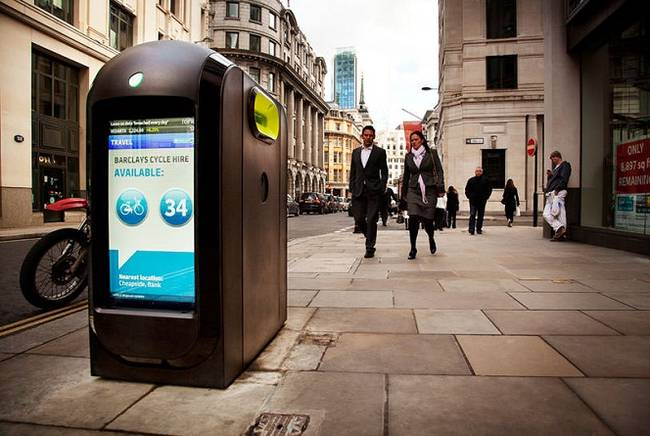
\includegraphics[scale=0.5]{pictures/London_Thank_Pod_Renew.jpg}
    \caption{\glqq{}Smart bin\grqq{} von \glqq{}Renew\grqq{} in London. Diese \glqq{}Smart Trashes\grqq{} waren Ihrer Zeit voraus.}
    \label{fig:LondonSmartBin}
\end{figure} 
Medienberichten zufolge haben diese Pods alle vorbeigehenden \gls{wlan}-Geräte anhand der MAC-Adresse getrackt, was den Bürgern von London missfiel. Deshalb stoppte die Stadt schliesslich ein Jahr später diese Mülleimer\autocite{market:LondonBinsStop}, was die Firma in den finanziellen Ruin trieb\autocite{market:LondonBinRuin}.
  Ob diese smarten Eimer den Füllstand auch überprüften, ist in den heute noch verfügbaren Berichten leider nicht mehr nachvollziehbar. Auch die Homepage des Unternehmens (\url{renewlondon.com}) ist nicht mehr erreichbar. Offenbar war das Unternehmen damals der Zeit voraus. Heutzutage gehört das Erfassen von MAC-Adressen in vielen Einkaufszentren und anderen Orten zur Tagesordnung. 
  \item Auch im Jahre 2013 haben Studenten von der University of Maryland einen \glqq{}Smart Trash\grqq{} namens \glqq{}Sorting Trash Can\grqq{}\autocite{market:sortingTrashCan} entwickelt, welcher den Müll trennt. Sie verlassen sich dabei auf das Geräusch, welches der Abfall beim Aufprall auf eine Platte macht. An Füllstandüberprüfung haben die Studenten jedoch nicht gedacht.
  \item In China wurden in 2015 \glqq{}King Kong-Trashes\grqq{}\autocite{market:ChinaTrash} installiert, welche laut Medien Feuer- und Bombensicher sind und welche die Müllkategorie mit Radar-Scanning erkennen und anhand dieser sortieren. Weiter sind die Eimer mit einem \gls{wlan}-Hotspot ausgerüstet und angeblich versorgt ein Solarpanel diese Eimer mit Strom. Vermutlich wird der Mülleimer über 2/3/4G-Netze kommunizieren um den \gls{wlan}-Hotspot zur Verfügung zu stellen. Eine Kommunikationsleitung wäre damit schon verfügbar um einen gemessenen Füllstand zu übermitteln. Eine Medienmitteilung von einem andern Portal beschreibt auch genau dies\autocite{market:ChinaTrash2}.
  
  \item Auch in näherer Umgebung gibt es smarte Abfalleimer: In Freiburg wurden testweise vier \glqq{}Big Belly\grqq{}-Mülleimer installiert\autocite{market:BigBelly}. Diese Eimer haben eine solarbetriebene Müllpresse, welche laut eigenen Angaben das Müllkontingent des Eimers um das siebenfache erhöht. Die Eimer können auch mit einer SIM-Karte ausgerüstet werden und so ihren Füllstand über das Mobilnetz via E-Mail mitteilen.
\end{itemize}

Bis zu dieser Recherche schien noch kein Unternehmen auf die Idee gekommen zu sein, Mülleimer \glqq{}nur\grqq{} mit einem Füllstandmesser auszurüsten. Stattdessen werden immer gleich \glqq{}Smart-Monster\grqq{} ausgeliefert, welche natürlich auch dementsprechend viel kosten. Unsere Idee, einen kleinen Füllstandsensor für bestehende Mülleimer ist also immer noch auf gutem Wege. Erst als wir schon bedeutend weiter in unserer Arbeit fortgeschritten waren, entdeckten wir das Unternehmen Enevo\autocite{market:Enevo}. Diese finnische Firma entwickelt ebenfalls einen kleinen Sensor, welcher via Ultraschall den Status eines Mülleimers misst. Was ihren Sensor jedoch teuer machen wird: die Übermittlung über das herkömmliche Mobilnetz. Hier hat unsere Idee also immer noch einen Trumpf im Ärmel und gleichzeitig zeigt Enevo, dass unsere Idee definitiv eine gesuchte Lösung ist.
\newpage

\section{Feldstudie}
Der Use Case war nun entwickelt und der Markt recherchiert. Damit die Idee aber weiterentwickelt werden konnte, war es notwendig, Personen aus dem Umfeld zu befragen, welche Erfahrung in diesem Bereich haben. Für den Tresh eignet sich natürlich ein Tiefbauamt, welches die Müllentsorgung einer Stadt verwaltet. Wir haben aufgrund des Wohnsitzes von Simon Wittwer beim Tiefbauamt Thun nachgefragt. Das Tiefbauamt hat sich freundlicherweise für ein Interview zur Verfügung gestellt.

\subsection{Tiefbauamt Thun}
Das Tiefbauamt Thun hat zwei Abteilungen, welche sich mit Abfall auseinandersetzen: Das Strasseninspektorat und die technischen Betriebe.

Das Strasseninspektorat hat die Verantwortung für saubere Strassen und in diesem Zusammenhang auch für die Leerung und Reinigung der über 500 Mülleimer und über 150 \glqq{}Robidogs\grqq{} in der Stadt. Im Sommer stellen sie jeweils noch einige Mülleimer zusätzlich auf, um dem in dieser Saison erhöhten Müllaufkommen entgegenzuwirken. Sie haben Leerungstouren nach Region und Müllaufkommen aufgeteilt. In den Ballungszentren müssen sie teilweise zweimal täglich die Eimer leeren. In den abgelegeneren Orten ist eine Leerung teilweise nur alle 14 Tage nötig. Teilweise müssen die Müllmänner vorbeigehen, auch wenn die Eimer noch nicht voll sind, denn als Strassenreiniger müssen sie auch die nahe Umgebung des Eimers sauber halten. An den Orten mit dem höchsten Müllaufkommen sind zwei Mülleimer des Produktes \glqq{}Big Belly\grqq{} im Einsatz. Das sind dieselben Mülleimer wie in Freiburg im Einsatz sind. Die Übermittlung des Füllstandes interessiert sie zurzeit jedoch noch nicht. Sie verwenden diese Eimer hauptsächlich aufgrund der integrierten Müllpresse, um somit die Leerungs-Zyklen dank erhöhter Kapazität zu senken. Dass sie die Füllstände dieser beiden Eimer nicht über Fernzugriff abrufen wollen, kommt aber nicht von Desinteresse an solchen Technologien, sondern macht bei zwei Eimern einerseits noch keinen Sinn und andererseits befinden sich die Eimer sowieso an den Orten, wo die Leerungen täglich stattfinden.

Die technischen Betriebe haben einen Disponent Abfallentsorgung. Dieser organisiert und verwaltet die Container- und Unterflur-Anlagen, welche die Stadt für die Hauskehricht- und Papierentsorgung betreibt. Glas und Aluminium wird interessanterweise nicht von der Stadt, sondern von der Privatfirma AVAG übernommen.
Auch bei diesen Containern hat das Tiefbauamt bereits Erfahrungen mit ersten \gls{iot}-Versuchen gemacht. vor vier Jahren hatte eine Firma Ultraschallsensoren zur Messung der Füllstände installiert. Leider ohne Erfolg, die Sensoren lieferten falsche Messresultate und meldeten, dass der Container voll sei, auch wenn er erst halbvoll war. Das vermutlich aufgrund von \glqq{}Bergbildung\grqq{} innerhalb des Containers. Das heisst, der herabfallende Müll häufte sich in Form eine Pyramide auf, dessen Spitze vom Sensor erfasst wurde und deshalb den Container als voll meldete. Aufgrund dieses Misserfolges war das Amt natürlich enttäuscht über die Technologie und daher etwas skeptisch gegenüber integrierter Sensoren geworden. Sie verstehen aber auch, dass in vier Jahren die Technologie wieder Fortschritte gemacht hat und sind deshalb nicht abgeneigt gegenüber neue Sensoren.

\subsection{Resultate aus dem Interview}
Das Konstruktive Interview mit den Herren des Tiefbauamts brachte uns viele neue Inputs, welche wir für den weiteren Verlauf des Projekts mitnehmen.
Da es beidseitig nicht ganz einfach war einen Termin zu finden, mussten wir allerdings bereits vor dem Interview mit der Entwicklung des Prototyps beginnen. Deshalb konnten wertvolle Informationen und das Feedback zu unserer Idee von den Herren leider nicht mehr in den Prototypen einfliessen. Wir nehmen dieses Wissen aber mit für einen eventuellen Nachfolgeprototypen in der Bachelorarbeit. Folgende Punkte halten wir fest:
\begin{itemize}  
  \item Für ein Strasseninspektorat spielt nicht nur der Füllstand eines Mülleimers eine Rolle. Auch die Umgebung um den Mülleimer muss sauber sein. Optimal wäre dazu natürlich eine Kamera, welche die Umgebung periodisch fotografiert. Energietechnisch und für das Übertragen der Daten ist eine Kamera jedoch suboptimal und es käme sofort die Frage auf, wo die Kamera aufgestellt werden kann. Statt einer Kamera könnte jedoch ein Feedback-System beim Eimer eingebaut werden. Vorbeigehende Passanten treffen eine Frage auf dem Eimer an: \glqq{}Ist's hier sauber?\grqq{} und können mit einem \glqq{}Daumen hoch\grqq{}- oder \glqq{}Daumen runter\grqq{}-Knopf darauf antworten. Dadurch könnten quasi die Passanten die Augen für das Reinigungsteam spielen.
  \item Für die Müllmänner wäre trotz der Füllstandüberwachung durch Fernzugriff auch eine lokale Füllstandanzeige sehr praktisch. Wenn sie gerade vor Ort sind müssten sie nicht den Müll öffnen um dessen Füllstand zu überprüfen, sondern könnten nur die Anzeige (beispielsweise eine LED) kontrollieren. Wenn jeder Müllmann ein Smartphone mit einer Leerungs-App hat relativiert sich dieser Punkt natürlich wieder.
  \item Die Sensoren müssen vor Vandalen und Witterungsschäden geschützt werden. Da die Mülleimer jeweils mit Hochdruckreinigern geputzt werden, muss der \gls{iotk} auch wasserdicht sein.
  \item Für Container ein einzelner Ultraschallsensor nicht ausreichend. Entweder müssen mehrere  Ultraschallsensoren oder andere Messemethoden eingesetzt werden.
\end{itemize}

\chapter{Protoyp}
\section{Übersicht}
Der Tresh-Prototyp besteht aus einem Libelium Waspmote als \gls{iotk}, einem Raspberry Pi 3 als \gls{iotg} und \gls{siot} als \gls{iotp}.
\begin{figure}[H]
     \centering
        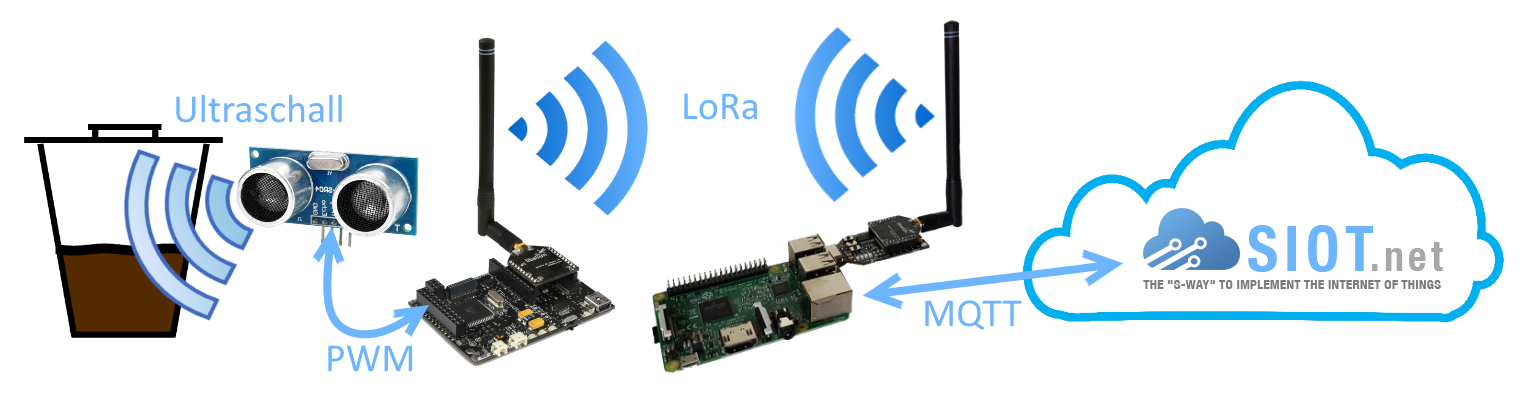
\includegraphics[width=1.0\textwidth]{pictures/PrototypeConcept.png}
    \caption{Gesamt-Architektur des Prototyps inklusive Schnittstellen}
    \label{fig:PrototypeConcept}
\end{figure}
Die Entwicklung des Prototyps bestand aus drei Teilen. Der Erste Teil war evaluation von geeigneter Hardware für den \gls{iotk} und den \gls{iotg}. Als nächstes musste die Hardware zusammengebaut werden, wobei hier ein massgeschneidertes Gehäuse per 3D-Druck entwickelt wurde. Parallel zur Entwicklung der Hardware wurde die Software für den Raspberry Pi und den Waspmote entwickelt. 

\section{Hardware}

\subsection*{\gls{iotk}-Evaluation}
Für die Evaluation des Knoten wurden verschiedene Embedded-Plattformen in Betracht gezogen. Da dies noch vor der definitiven Entscheidung für LoRa geschah, sind bei den Plattformen auch andere Funktechnologien berücksichtigt worden.

\subsubsection*{Sming}
Sming basiert auf dem TWX51-Sensor Node, welcher von Daniel Meer an der BFH/TI  entwickelt wurde. Herr Meer beschreibt den TWX51 wie folgt: 
\begin{quote}
\textit{Der TXW51 ist ein kleiner und energiesparender Sensorknoten, der als Basis für zukünftige Projekte verwendet werden
kann. Er kommuniziert über Bluetooth Smart und enthält einen Sensor zur Messung der Beschleunigung. Die Firmware kann einfach für neue Anforderungen modifiziert werden.}\autocite{bfh:TXW51}
\end{quote}

\begin{figure}[H]
     \centering
        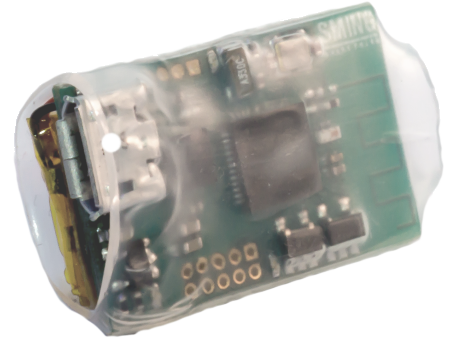
\includegraphics[scale=0.6]{pictures/Sming.png}
    \caption{Sming mit Akku bestückt}
    \label{fig:Sming}
\end{figure}

\textbf{Vorteile}
\begin{itemize}
\item Eigenentwicklung der BFH/TI, Wissen komplett inhouse vorhanden
\item Optimiert für tiefen Energieverbrauch
\item sehr kleine Grösse (2.5cm x 1.7cm)
\item hat integrierte \gls{ble}-Schnittstelle
\end{itemize}
\textbf{Nachteile}
\begin{itemize}
\item kann zwar über Interrupts aufgeweckt werde, hat jedoch kein RTC
\item hat nur 3V-Spannung (nicht 3.3V), dadurch inkompatibel zu 5V-Sensoren
\item nur kurze Funk-Distanzen aufgrund von BLE
\item keine Lang-Distanz-Funk-Technik
\end{itemize}

\newpage

\subsubsection*{Tiny-Mesh}
Tiny-Mesh ist das Produkt des gleichnamigen Unternehmens aus Norwegen. Die Idee hinter diesm Produkt ist ein selbst-formendes und selbst-heilendes Sensor-Mesh-Netzwerk zu konstruieren, welches die Sensordaten der einzelnen Knoten an eine Cloud anbindet. Die Knoten basieren auf Modulen von Radiocraft, welche den proprietären Tiny-Mesh-Ptrotokoll-Stack implementieren. Für die Evaluation erhielten wir ein Starter-Kit zum testen.

\begin{figure}[H]
     \centering
        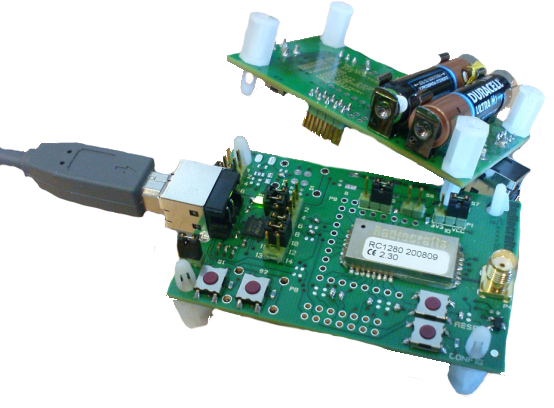
\includegraphics[scale=0.5]{pictures/TinyMesh.png}
    \caption{Radiocraft-Modul und die Batteriehalterung auf der Unterseite}
    \label{fig:TinyMesh}
\end{figure}

\textbf{Vorteile}
\begin{itemize}
\item Mesh-Netzwerk ermöglicht Erweiterung durch nodes
\item Mesh-Netzwerk ist selbst-heilend
\item Mesh-Netzwerk ist selbstkonfigurierend
\end{itemize}
\textbf{Nachteile}
\begin{itemize}
\item Proprietärer TinyMesh-Protokoll-Stack
\item Module sind nicht Programmierbar, Logik muss von externem Plattform gemacht werden
\item hoher Energieverbrauch durch Mesh-Topologie
\end{itemize}

\newpage

\subsubsection*{Waspmote}
Waspmote ist eine Mikrocontroller-Plattform von der Spanischen Firma Libelium. Die Plattform ist Modular aufgebaut und unterstützt verschiedenste Funktechniken wie Zigbee, GSM und unter anderem auch LoRa. Durch das modulare Design können Funkchips schnell ausgewechselt werden. Die Plattform ist praktisch um Prototypen zu erstellen, wird von Libelium aber auch als Produkt in Kombination mit über 100 verschiedenen Sensoren vertrieben.
\begin{figure}[H]
     \centering
        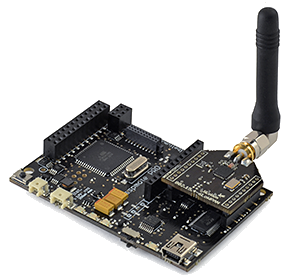
\includegraphics[scale=1.0]{pictures/Waspmote.png}
    \caption{Libelium Waspmote}
    \label{fig:Waspmote}
\end{figure}

\textbf{Vorteile}
\begin{itemize}
\item Modular aufgebaut und ideal für einen Prototyp
\item unterstützt viele Funk-Technologien
\item hat einen RTC und kann den Mikrocontroller deaktivieren um Energieverbrauch zu minimieren. (0.6µA Verbrauch wenn nur RTC in Betrieb)
\item viele GPIOs 
\end{itemize}
\textbf{Nachteile}
\begin{itemize}
\item relativ gross (7.3cm x 5.1cm)
\item teuer (allein ein Waspmote kostet 163 Euro, stand 24.06.2016)
\item verhältnismässig hoher Energieverbrauch, wenn in Betrieb (15mA) und nicht in sleep. Die Ursache davon sind jedoch die vielen GPIos was gleichzeitig ein Vorteil ist
\end{itemize}

\subsection*{Entscheidung}
Mit der Entscheidung, das Netzwerk auf LoRa aufzusetzen, war die Entscheidung schon fast getroffen. Der Sming hätte zwar auch mit einem LoRa-Chip verbunden werden können, dies wäre jedoch ein Projekt für Studenten der Elektrotechnik. Das Waspmote überzeugt mit seiner Modularität, dem vorhandensein eines RTCs und nicht zuletzt auch damit, dass die Plattform auch schon von Roger Jaggi und Pascal Bohni erfolgreich eingesetzt wurde.

\subsection{Distanz-Sensor}
Wie in Kapitel \ref{chapter:devOfUseCase} beschrieben wird der Füllstand des Mülleimers durch Distanz mittels Ultraschall gemessen. Für diese Messung wird der Ultraschall-Sensor "HC-SR04" eingesetzt. Er hat einen Messbereich von 2 bis 500cm. Dieser Bereich beinhaltet alle Distanzen, welche in allen handelsüblichen Mülleimern gemessen werden können. Falls eine Version für Container erstellt werden sollte, müsste ein Sensor mit grösserem Messbereich verwendet werden. 
\begin{figure}[H]
     \centering
        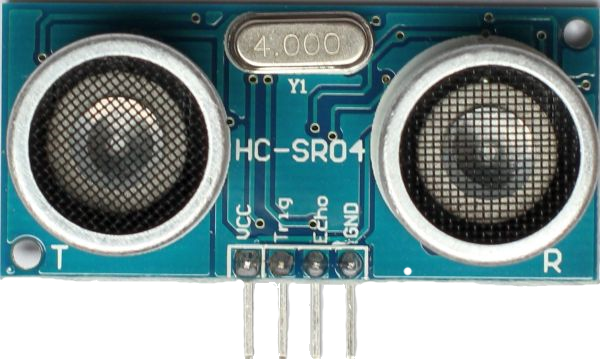
\includegraphics[scale=0.3]{pictures/HC-SR04.png}
    \caption{Ultraschall-Sensor HC-SR04}
    \label{fig:HCSR04}
\end{figure}

\subsection{\gls{iotg}}
Als \gls{iotg} wurde ein Raspberry Pi 3 eingesetzt. Dieser kleine, flexible Einplatinencomputer bietet viele Schnittstellen an, lässt die Wahl zwischen verschiedenen Betriebssystemen und hat eine grosse Community. Für den Anwendungsfall des Tresh-Gateways sind die Netzwerkschnittstellen, um das Gateway mit dem Internet zu verbinden und die USB-Schnittstellen, um das Waspmote Gateway\footnote{Waspmote Gateway: \url{http://www.libelium.com/products/waspmote/interfaces/\#gateway_marker} Slide 11} an das Raspberry Pi anzuschliessen, essenziell. Das Raspberry Pi 3 bietet dazu zusätzlich zur Ethernet Schnittstelle auch gleich ein fest eingebautes \gls{wlan} Modul an, was viel flexibilität bei der Platzierung des Gateways ermöglicht. Nichtsdestotrotz ist natürlich die Ethernet-Schnittstelle zu bevorzugen, da diese eine stabilere Netzwerverbindung zur Verfügung stellt als die \gls{wlan} Schnittstelle. 

\section{Hardware-Implementation}
Nachdem die die Ware verfügbar war, wurde ein erster Proof-of-Concept aus Holz und einem grossen Breadboard erstellt. Dieser Prototyp hatte Hardwaremässig bereits die volle Funktion. Softwaremässig konnte er ganz rudimentär die gemessene Distanz via LoRa versenden.

\begin{figure}[H]
     \centering
        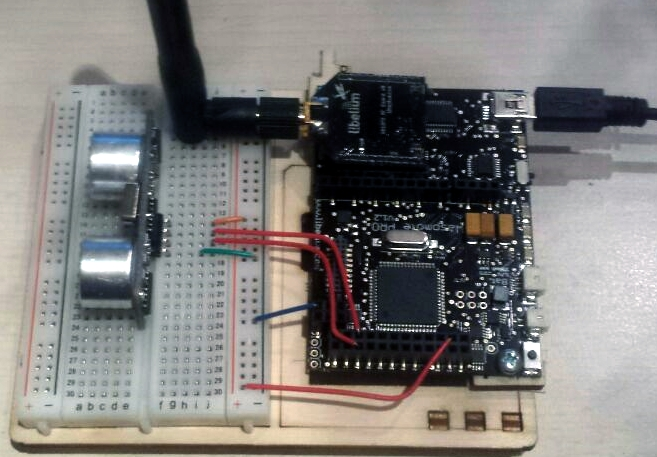
\includegraphics[scale=0.6]{pictures/Prototype1.jpg}
    \caption{Erster Prototyp des \gls{iotk}}
    \label{fig:HCSR04}
\end{figure}

Damit dieser Knoten jedoch in einem Mülleimer eingebaut werden kann, braucht er ein schützendes Gehäuse, damit er einerseitz nicht einfach verschmutzt und andereseits stabil im Eimer montiert werden kann. Mithilfe der Opensource-Software OpenSCAD konstruierten wir ein zweistöckiges Gehäuse. Im oberen Teil ist der Platz für das Waspmote und ein kleines Breadboard für den Ultraschall-Sensor, im unteren Stock ist Platz für die Batterie. Die Batterie ist ein 6600mAh-Akku, welcher von Libelium für das Waspmote angeboten wird. 
 
\begin{figure}[H]
     \centering
        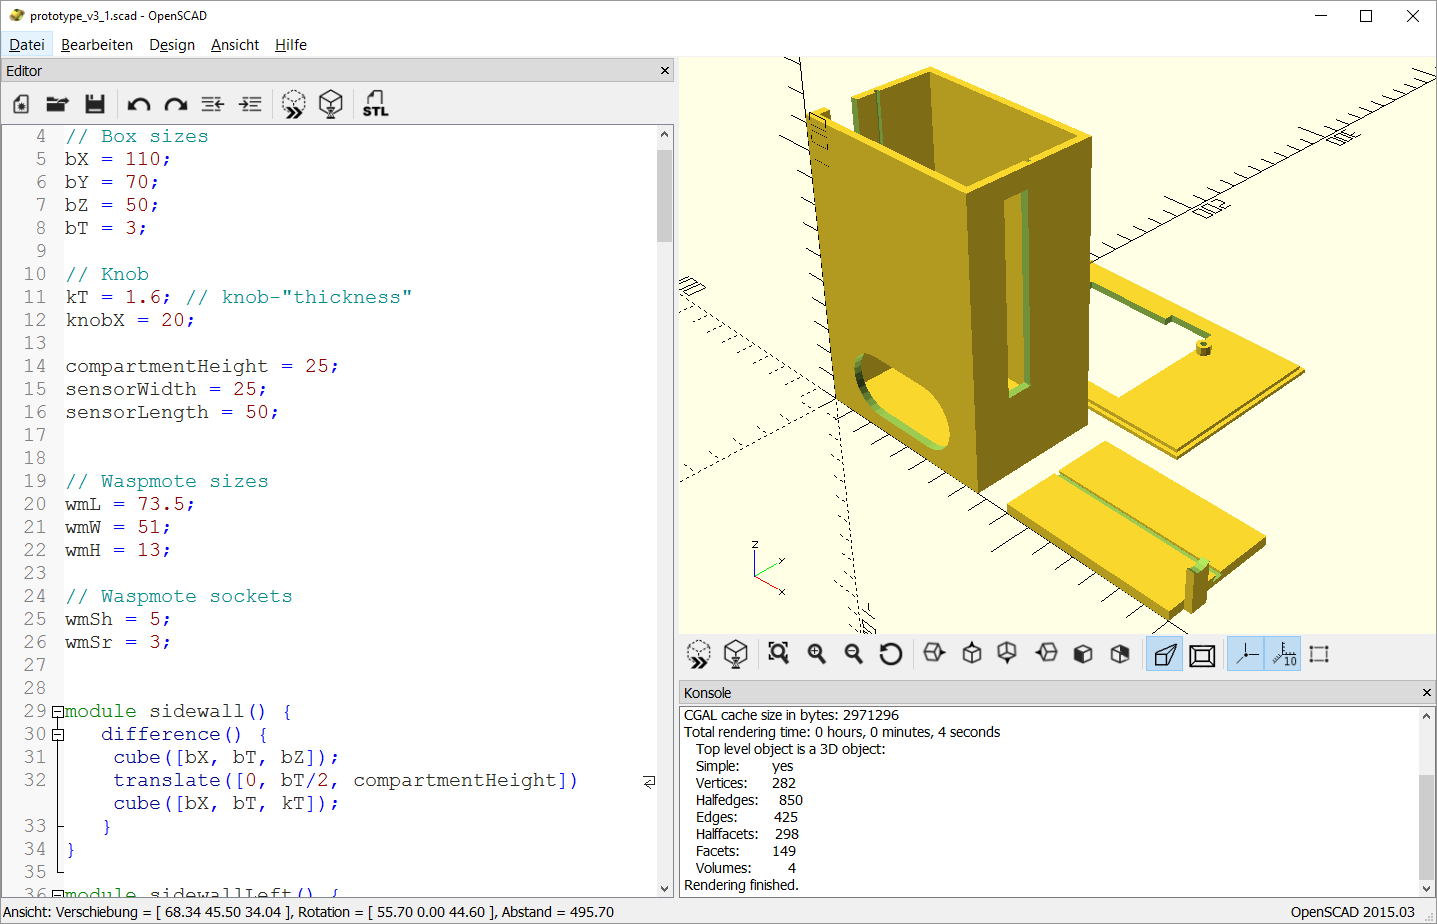
\includegraphics[width=1.0\textwidth]{pictures/OpenSCAD.png}
    \caption{Entwicklung des Gehäuses für den Prototyp}
    \label{fig:OpenSCAD}
\end{figure}

Das Konzept des Gehäuses ist ein Schubladensystem. Das bedeutet, dass die Platine, welche die beiden Kammern des Gehäuses trennt, wie ein Schlitten in das Gehäuse einfahrbar ist. Auf dieser Platine wir auch Was Waspmote und der Sensor montiert. Dies hat zum Vorteil, dass bei einem Wartungszugriff die ganze Hardware einfach aus dem Gehäuse gezogen werden kann.
Das Gehäuse druckten wir auf einem Ultimaker 3D-Drucker aus. Es benötigte mehrere Testdrucks und verschiedenste Anpassungen am Plan bis das Gehäuse mit allen Komponenten zusammenpasste. Besonders delikat war das Schubladensystem, da der Schlitten mit 1mm Dicke nur gerade das zehnfache der Genauigkeit des 3D-Druckers ist.

\begin{figure}[H]
     \centering
        \includegraphics[width=0.55\textwidth]{pictures/3D-Print.jpg}
    \caption{Druck eines Gehäuse-Prototyps mit Ultimaker}
    \label{fig:3D-Print}
\end{figure}

Nachdem alle Gehäusekomponeten zusammenpassten und das Waspmote und das Breadboard montiert werden konnten, starteten wir die "Massenproduktion". Mit Massenproduktion ist in diesem Zusammenhang eine Stückzahl von 3 gemeint.

\begin{figure}[H]
     \centering
        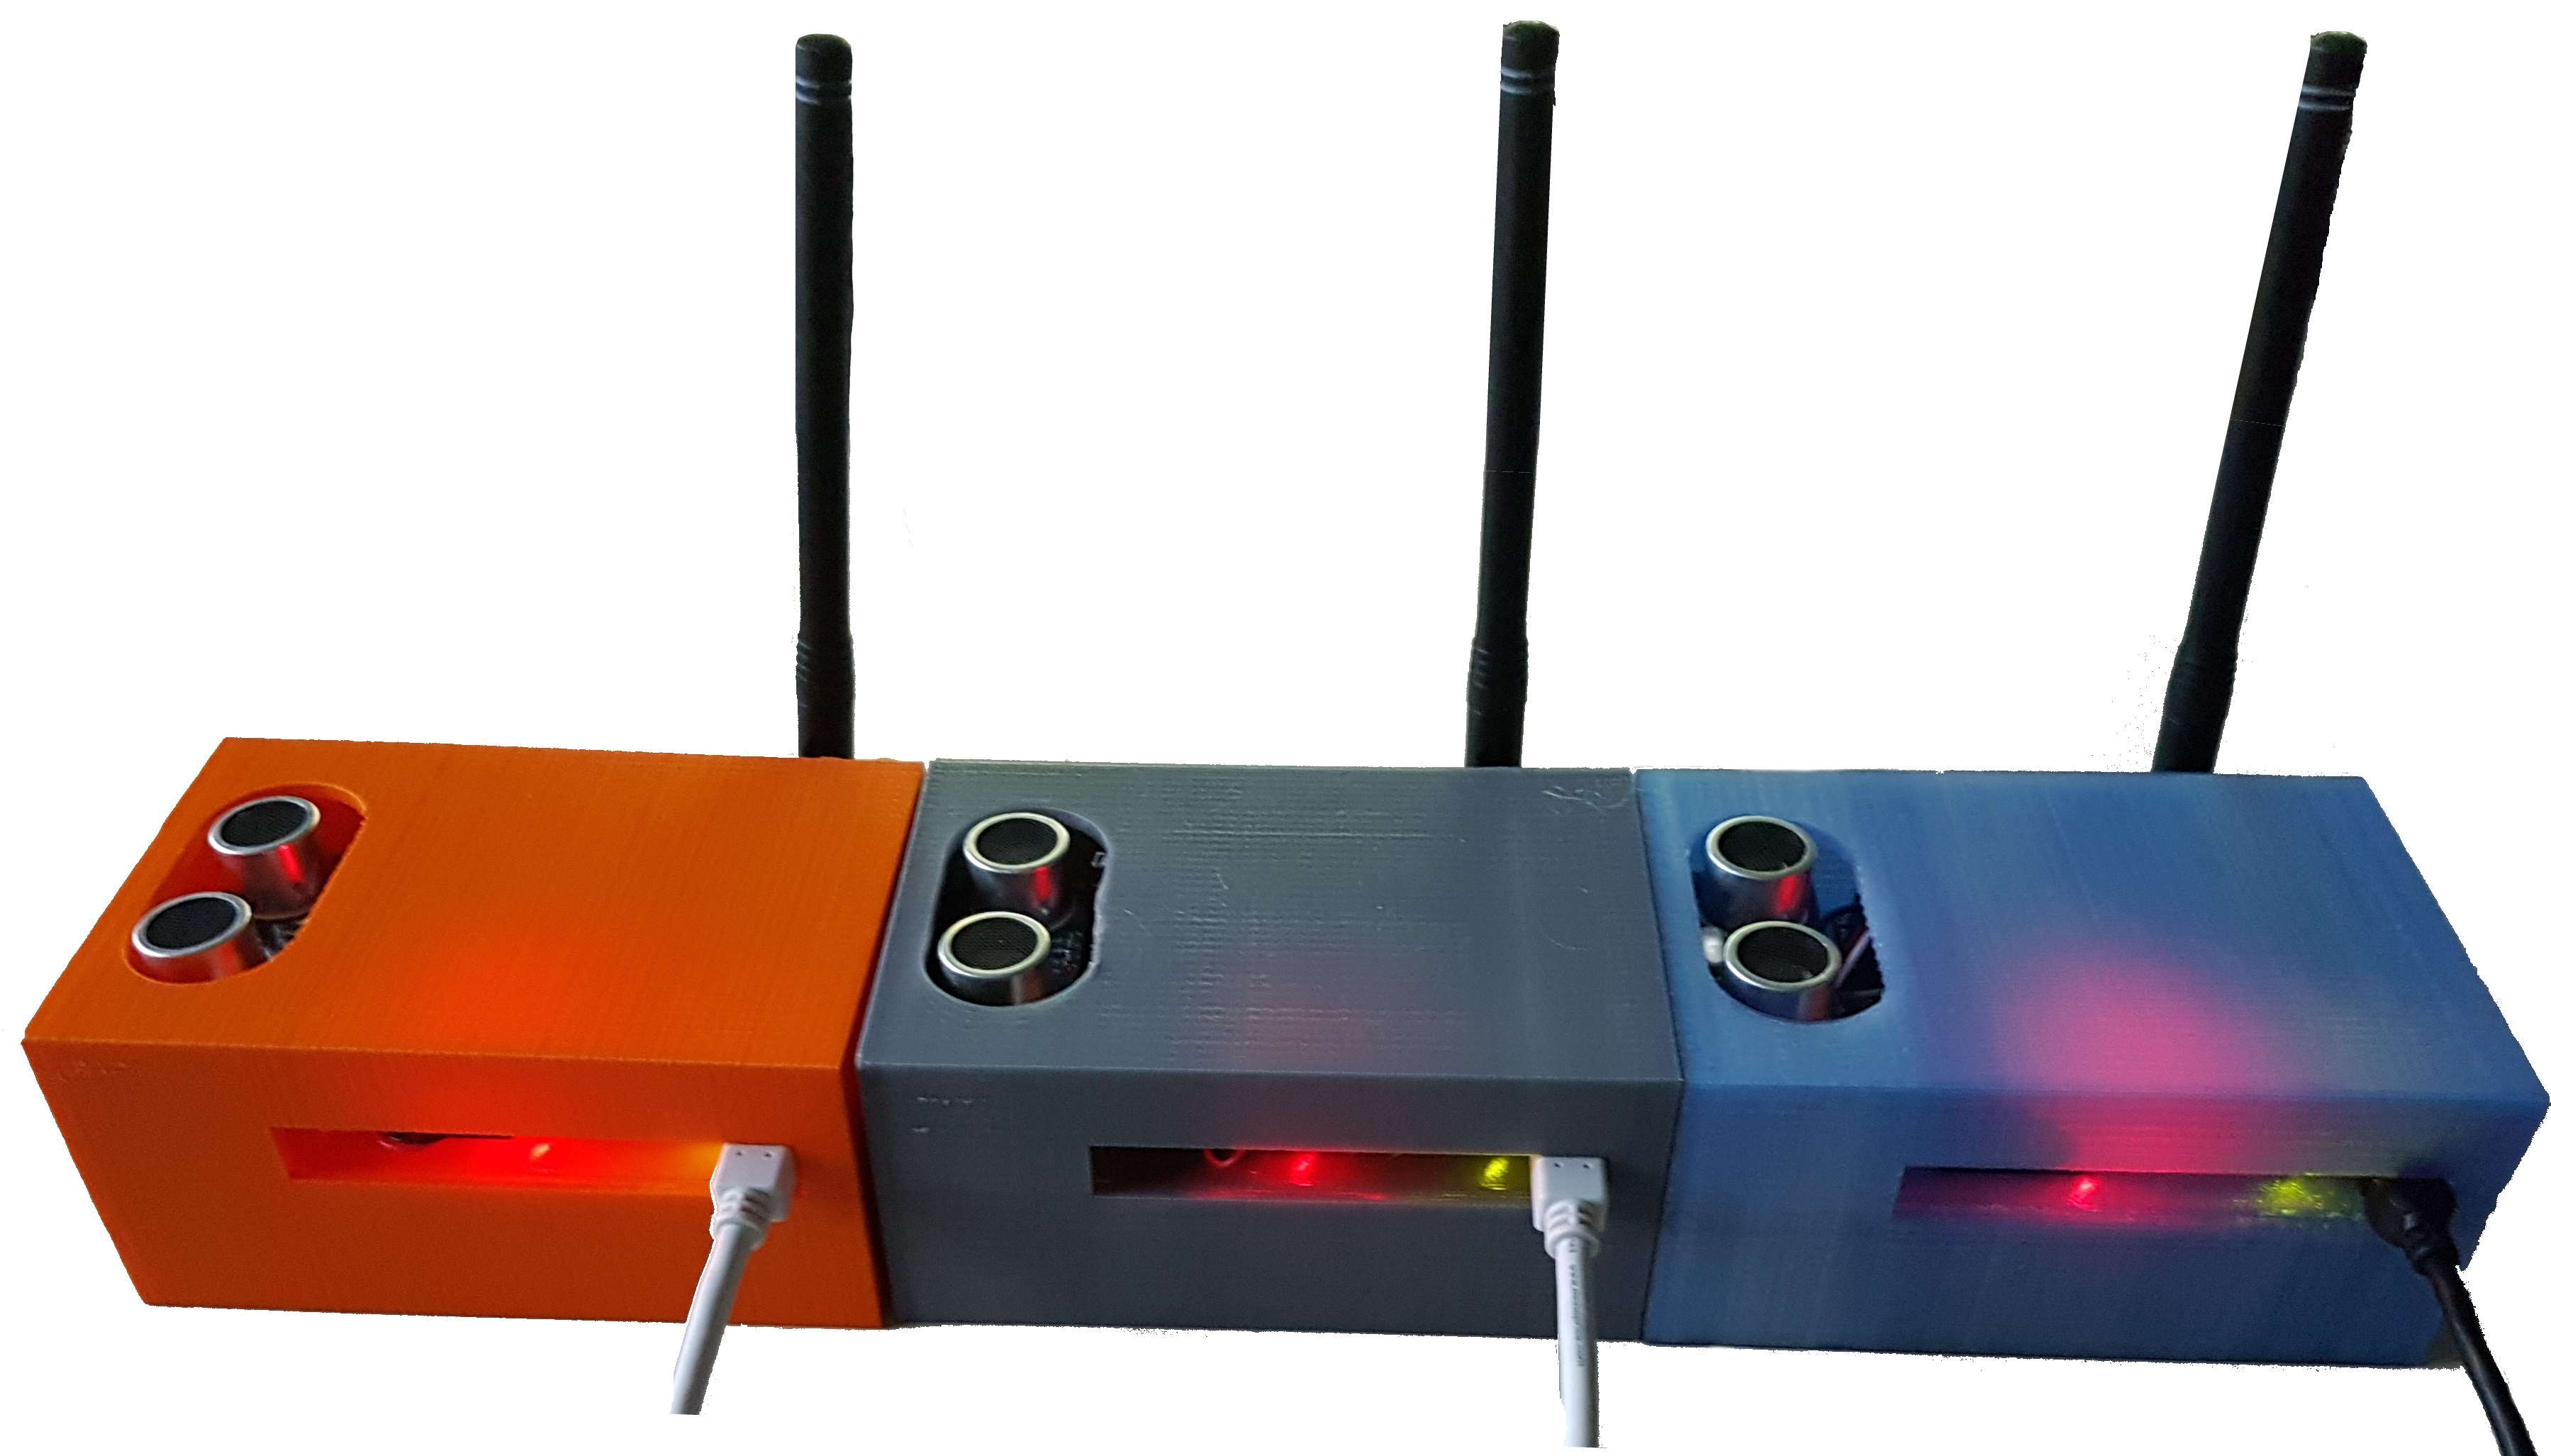
\includegraphics[width=0.8\textwidth]{pictures/Massproduction.jpg}
    \caption{Die 3 fertigen Prototypen}
    \label{fig:3-Prototypes}
\end{figure}

Als nächstes mussten die Prototypen natürlich auch in den Einsatz gebracht werden. Als Testumfeld wurden zusammen mit Herr Danuser die PET-Eimer des Rolex-Gebäudes der BFH in Biel ausgewählt. Herr Danuser holte bei Herrn Schüpbach, dem Leiter des Hausdienstes, die Erlaubnis ein. Dieser erlaubte uns, im PET-Eimer in der Mensa und im PET-Eimer im 5. Stock des Gebäudes einen Sensor zu platzieren.

\subsection*{Installation}
Am Freitag, den 10. Juni 2016 konnten wir die Sensoren an ihren Standorten platzieren. Für den Raspberry Pi mit dem Waspmote-Gateway stellte uns Herr Danuser sein Büro zur Verfügung, damit dieser eine unversiegende Energiequelle sowie Ethernet-Anschluss hat.
Dabei mussten wir feststellen, dass definitiv der Spreizfaktor von LoRa benötigt wird, damit das Gateway den Sensor in der Mensa noch "hört". Der Sensor sendet mit 7dB Ausgangsleistung, das Gateway hat mit dem maximalen Spreizfaktor von LoRa eine Empfindlichkeit von -136dBM. Dies ergibt ein Powerbudget von 143dB, welches auch ziemlich ausgenutzt wird. Das Gateway sendet jeweils eine Ack-Bestätigung, wenn ein Sensor ein Packet versandt hat. Damit diese Ack-Packete garantiert ankommen, sendet das Gateway mit 14dB.

\begin{figure}[H]
     \centering
        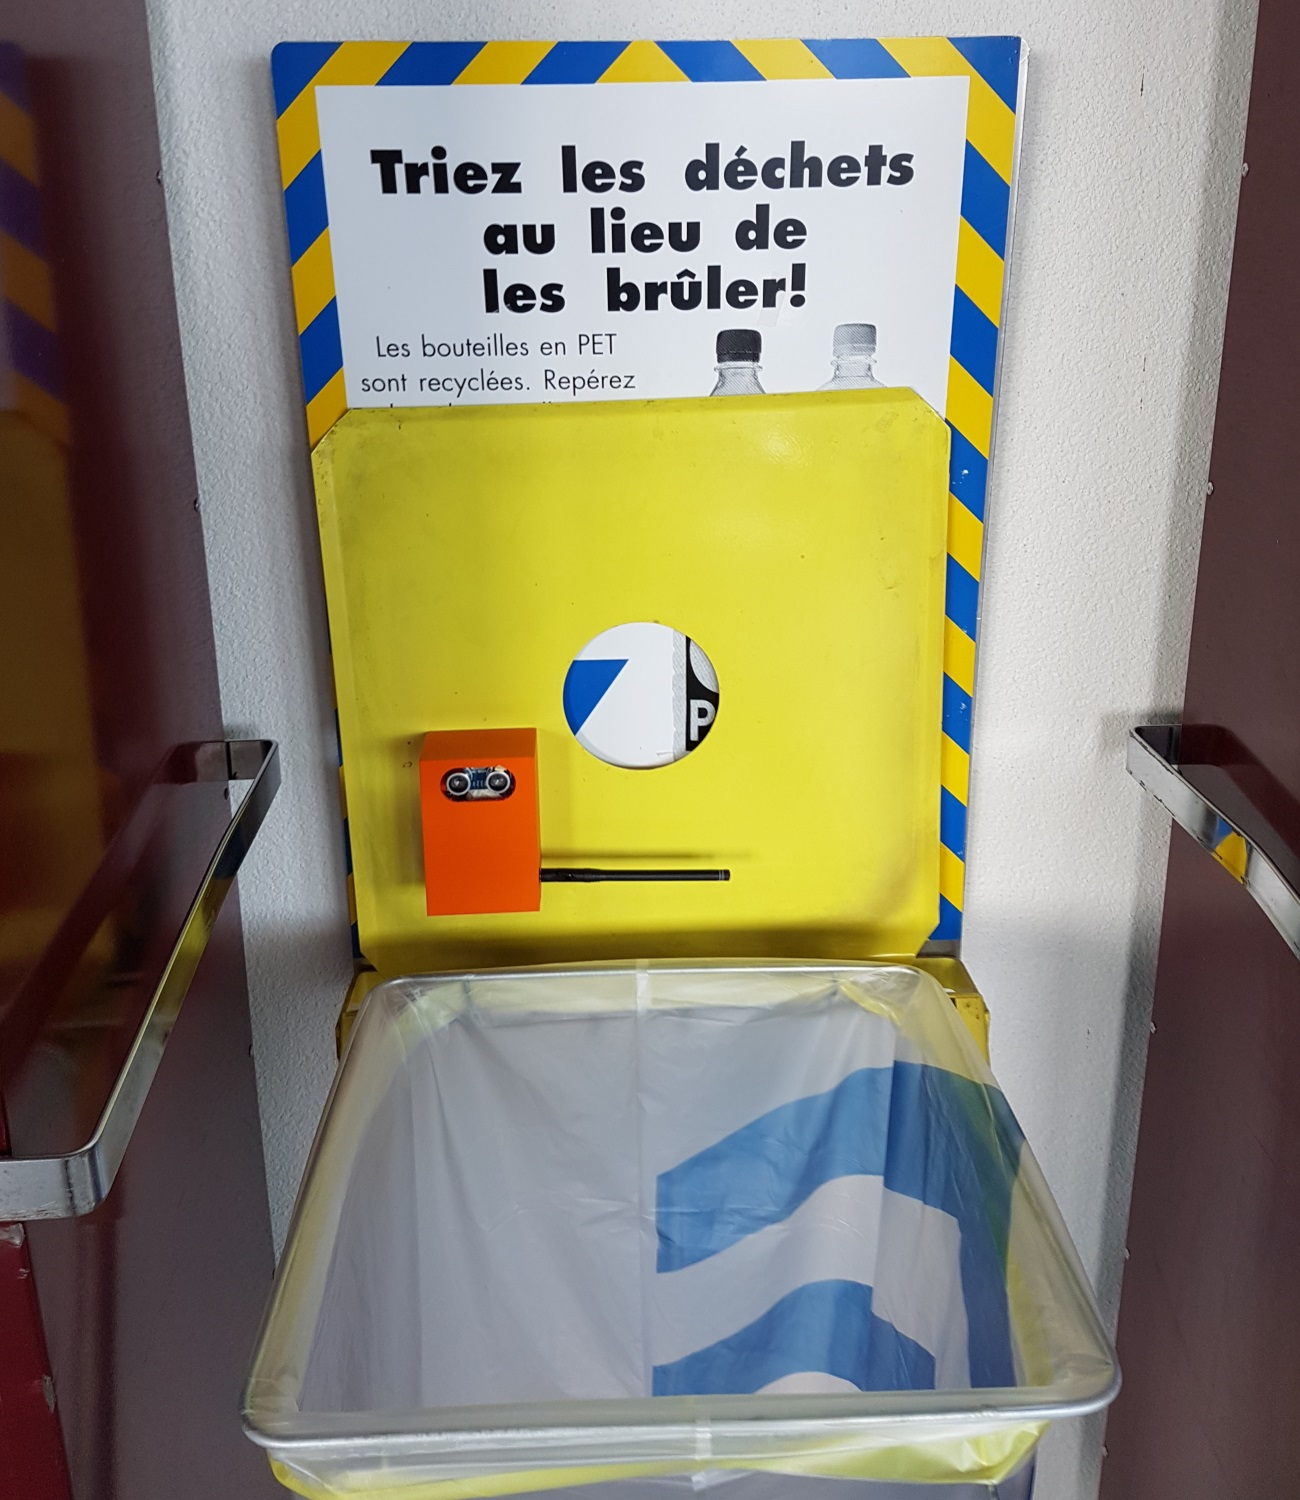
\includegraphics[width=0.7\textwidth]{pictures/Tresh-Deployed.jpg}
    \caption{Der am aufgeklappten Deckel des PET-Eimers in der Mensa befestigte Prototyp}
    \label{fig:3-Prototypes}
\end{figure}

Der zweite Sensor im 5. Stock konnte leider nicht installiert werden. Der dortige Eimer ist komplett aus Metall konstruiert. Sobald der Sensor im Eimer eingeschlossen ist, wird sein Signal durch Reflexionen und Dämpfung des Eimers um ungefähr 45dB gedämpft. Das restliche Powerbudget von 98dB reicht leider nicht aus um das Gateway in Herrn Danuser's Büro zu erreichen. Der Prototyp bräuchte ein Koaxialkabel, damit wir seine Antenne ausserhalb des Eimers befestigt werden könnte und nur durch das Koaxial-Kabel zum Prototypen im Eimer verbunden wäre.


\section{Software}

\subsection{Waspmote als \gls{iotk}}


\subsection{Raspberry Pi als \gls{iotg}}

Die Hauptfunktion eines \gls{iotg} ist es ein Sensor Netzwerk mit einer \gls{iotp} zu verbinden. Genau diese Funktion wurde auf dem Raspberry Pi durch zwei Softwarekomponenten implementiert:

\begin{enumerate}
	\item tresh-lora-gateway - Sensordaten aus dem \gls{lora}-Netzwerk auf dem Waspmote Gateway empfangen.
    \item tresh-siot-gatway - Sensordaten des Waspmote Gateway an die \gls{siot} \gls{iotp} senden.
\end{enumerate}

Der dazugehörige Quellcode ist im Anhang unter \ref{appendix:raspberrypi} aufgeführt.

\subsubsection*{tresh-lora-gateway}

Die Aufgabe dieser Softwarekomponente ist es die Sensordaten aus dem \gls{lora}-Netzwerk zu empfangen und über USB eine serielle Schnittstelle zu emulieren welche die Daten ausgibt.

\subsubsection*{tresh-siot-gatway}

Die Aufgabe dieser Softwarekomponente ist es die Sensordaten über die serielle Schnittstelle zu empfangen und über \gls{mqtt} an die \gls{siot} \gls{iotp} weiterzuleiten. In der Bachelor Thesis \autocite{bfh:optimizedDataTransmission} hat Roger Jaggi die \gls{nodejs}-Applikation siot.net-nodejs-api\autocite{bfh:siot.net-nodejs-api} geschrieben, welche die \gls{siot} Gateway API Spezifikation implementiert. Die tresh-siot-gatway Applikation baut auf dieser API auf. Wir haben zusätzlich das Auswählen und Auslesen des seriellen Ports und die Zuweisung der empfangenen Sensordaten an die entsprechenden, in \gls{siot} registrierten Sensoren implementiert. Diese Zuweisung geschieht aktuell lokal auf dem \gls{iotg} anhand der \gls{lora} Netzwerk Adresse der \gls{iotk}. In Zukunft sollte diese Zuweisung aber auf einer höheren Sofwareschicht implementiert werden.

\subsection{\gls{siot}}

\include{chapters/demo.md}

%---------------------------------------------------------------------------
% Statement
%---------------------------------------------------------------------------
\cleardoublepage
\phantomsection
\addcontentsline{toc}{chapter}{Selbständigkeitserklärung}
\chapter*{Selbstständigkeitserklärung}
\label{chap:selbstaendigkeitserklaerung}

\vspace*{10mm}
Wir bestätigen mit unseren Unterschriften, dass wir unsere vorliegende Bachelorthesis selbstständig durchgeführt haben. Alle Informationsquellen (Fachliteratur, Besprechungen mit Fachleuten, usw.) und anderen Hilfsmittel, die wesentlich zu unserer Arbeit beigetragen haben, sind in unserem Arbeitsbericht im
Anhang vollständig aufgeführt. Sämtliche Inhalte, die nicht von uns stammen, sind mit dem genauen Hinweis auf ihre Quelle gekennzeichnet.

\vspace{15mm}

\begin{tabbing}
xxxxxxxxxxxxxxxxxxxxxxxxx\=xxxxxxxxxxxxxxxxxxxxxxxxxxxxxx\=xxxxxxxxxxxxxxxxxxxxxxxxxxxxxx\kill
Ort, Datum:		\> Bern, \versiondate \\ \\
Namen:	\> Simon Wittwer 	\> Marc Zimmermann \\ \\ \\ \\
Unterschriften:	\> ......................................\> ...................................... \\
\end{tabbing}


%---------------------------------------------------------------------------
% Glossary
%---------------------------------------------------------------------------
\cleardoublepage
\phantomsection
% \addcontentsline{toc}{chapter}{Glossar}
% \renewcommand{\glossaryname}{Glossar}
% \printglossary
\printglossaries

%---------------------------------------------------------------------------
% Bibliography
%---------------------------------------------------------------------------
\cleardoublepage
\phantomsection
% \nocite{*}
\addcontentsline{toc}{chapter}{Literaturverzeichnis}
% \bibliographystyle{IEEEtranS}
% \bibliography{references/bibliography}{}
\printbibliography


%---------------------------------------------------------------------------
% Listings
%---------------------------------------------------------------------------
\cleardoublepage
\phantomsection
\addcontentsline{toc}{chapter}{Abbildungsverzeichnis}
\listoffigures

\cleardoublepage
\phantomsection
\addcontentsline{toc}{chapter}{Tabellenverzeichnis}
\listoftables

%---------------------------------------------------------------------------
% Index
%---------------------------------------------------------------------------
%\cleardoublepage
%\phantomsection
%\addcontentsline{toc}{chapter}{Stichwortverzeichnis}
%\renewcommand{\indexname}{Stichwortverzeichnis}
%\printindex

%---------------------------------------------------------------------------
% Appendix
%---------------------------------------------------------------------------
% \appendix
% \settocdepth{section}
% \include{appendix/example.md}

\begin{appendices}
\chapter{Quellcode \gls{iotk}}

\section{Waspmote}\label{appendix:waspmote}

\textbf{Auslesen der Sensordaten und Übertragung via LoRa}
\lstinputlisting[language=c,caption=tresh\_sensor\_node.pde]{source/tresh_sensor_node.pde}


\chapter{Quellcode \gls{iotg}}

\section{Waspmote Gateway}\label{appendix:waspmote-gateway}

\textbf{Sensordaten aus dem \gls{lora}-Netzwerk auf dem Waspmote Gateway empfangen}
\lstinputlisting[language=c,caption=tresh\_lora\_gateway.pde]{source/tresh_lora_gateway.pde}

\section{Raspberry Pi}\label{appendix:raspberrypi}

\textbf{Sensoren auf der \gls{siot} \gls{iotp} erstellen}
\lstinputlisting[language=JavaScript,caption=create-sensors.js]{source/create-sensors.js}

\textbf{Sensordaten des Waspmote Gateway an die \gls{siot} \gls{iotp} senden}
\lstinputlisting[language=JavaScript,caption=multi-sensor.js]{source/multi-sensor.js}

\section{Setup Raspberry Pi (RPI)}\label{setup-raspberry-pi-rpi}

\subsection*{Installation}\label{installation}

\begin{enumerate}
\def\labelenumi{\arabic{enumi}.}
\item
  Prepeare \texttt{cmdline.txt} of raspian image on sd card. Append the
  following:

\begin{verbatim}
ip=192.168.2.2
\end{verbatim}
\item
  (OSX) Internet Sharing WiFi to (Thunderbolt) Ethernet
\item
  Login to rpi (pw: raspberry)

\begin{verbatim}
ssh pi@192.168.2.2
\end{verbatim}
\item
  Set locales: Choose \texttt{en\_US.UTF8} in

\begin{verbatim}
sudo dpkg-reconfigure locales
\end{verbatim}
\item
  Set timezone: Choose \texttt{Zurich} in

\begin{verbatim}
dpkg-reconfigure tzdata
\end{verbatim}
\item
  Install required debian packages

\begin{verbatim}
aptitude install autossh git vim mosh htop # Not nodejs npm!!!
\end{verbatim}
\item
  Get latest Node.js debian package

\begin{verbatim}
wget http://node-arm.herokuapp.com/node_latest_armhf.deb
\end{verbatim}
\item
  Install Node.js

\begin{verbatim}
sudo dpkg -i node_latest_armhf.deb
\end{verbatim}
\item
  Checkout source code

\begin{verbatim}
mkdir ~/src
cd src/
git clone <tresh_repo_url>
\end{verbatim}
\end{enumerate}

\subsection*{Configuration}\label{configuration}

\subsubsection*{DNS}\label{dns}

Add following line to network interface in /etc/network/interfaces:

\begin{verbatim}
dns-nameservers 8.8.8.8 8.8.4.4
\end{verbatim}

\subsubsection*{SSH Reverse Tunnel}\label{ssh-reverse-tunnel}

\begin{enumerate}
\def\labelenumi{\arabic{enumi}.}
\item
  Add autossh-tresh systemd service

\begin{verbatim}
pi@raspberrypi:~ $ vim /etc/systemd/system/autossh-tresh.service

[Unit]
Description=Autossh tresh: Maintain a ssh reverse tunnel to a control server
# After=network.target
After=network-online.target

[Service]
# User=autossh
User=pi
Group=pi
# -p [PORT]
# -l [user]
# -M 0 --> no monitoring
# -N Just open the connection and do nothing (not interactive)
# LOCALPORT:IP_ON_EXAMPLE_COM:PORT_ON_EXAMPLE_COM
# ExecStart=/usr/bin/autossh -M 0 -N -q \
# -o "ServerAliveInterval 60" -o "ServerAliveCountMax 3" \
# -p 22 -l autossh remote.example.com \
# -L 7474:127.0.0.1:7474 -i /home/autossh/.ssh/id_rsa
TimeoutStartSec=3
TimeoutStopSec=3
ExecStart=/usr/bin/autossh -M 20000 -N -C -q \
-o "ServerAliveInterval 60" -o "ServerAliveCountMax 3" \
-p 22 -l tooreht tjmp -R 22000:localhost:22 \
-i /home/pi/.ssh/id_rsa
# ExecStart=/home/pi/scripts/autossh-tresh.sh
Restart=always

[Install]
WantedBy=multi-user.target
\end{verbatim}
\item
  Enable service

\begin{verbatim}
systemctl enable autossh-tresh.service
\end{verbatim}
\end{enumerate}

\subsubsection*{Detect Waspmote Gateaway USB via
udev}\label{detect-waspmote-gateaway-usb-via-udev}

\begin{enumerate}
\def\labelenumi{\arabic{enumi}.}
\item
  Add udev rule

\begin{verbatim}
pi@raspberrypi:~ $ vim  /etc/udev/rules.d/99-tresh.rules

SUBSYSTEM=="tty", ACTION=="add", \
ATTRS{manufacturer}=="FTDI", \
ATTRS{product}=="FT232R USB UART",\
  PROGRAM="/bin/systemd-escape \
  -p --template=tresh-gateway@.service $env{DEVNAME} $env{ID_FS_LABEL}",\
  ENV{SYSTEMD_WANTS}+="%c"
\end{verbatim}
\item
  Add tresh-gateway@ systemd service

\begin{verbatim}
pi@raspberrypi:~ $ vim /etc/systemd/system/tresh-gateway@.service

[Unit]
Description=tresh siot gateway
BindTo=%i.device
After=%i.device
After=rc-local.service

[Service]
Type=oneshot
TimeoutStartSec=0
ExecStart=/home/pi/scripts/tresh-gateway.sh /%I
# RemainAfterExit=yes
\end{verbatim}
\item
  Prepeare adding bash script

\begin{verbatim}
mkdir -p /var/log/tresh
touch /var/log/tresh/tresh-gateway.log
\end{verbatim}
\item
  Add bash script tresh-gateway.sh

\begin{verbatim}
vim ~/scripts/tresh-gateway.sh

#!/bin/bash
LOG=/var/log/tresh/tresh-gateway.log
cd /home/pi/src/tresh/gateway/tresh-siot-gateway
DEVNAME=$1 node multi-sensor.js $1 | tee $LOG
\end{verbatim}
\item
  Set permissions

\begin{verbatim}
chmod  u+x /home/pi/src/tresh/gateway/tresh-siot-gateway
\end{verbatim}
\item
  Check USB insertion via systemd journal

\begin{verbatim}
journalctl -xn --follow
\end{verbatim}
\end{enumerate}

\subsubsection*{Connect to WPA
Enterprise}\label{connect-to-wpa-enterprise}

\begin{enumerate}
\def\labelenumi{\arabic{enumi}.}
\item
  Add wpa configs

\begin{verbatim}
vim /etc/wpa_supplicant/wpa_supplicant.conf
country=CH
ctrl_interface=DIR=/var/run/wpa_supplicant GROUP=netdev
update_config=1

# Locked BFH network
network={
    ssid="bfh"
    key_mgmt=WPA-EAP IEEE8021X
    eap=PEAP
    auth_alg=OPEN
    phase1="peaplabel=0"
    phase2="auth=MSCHAPV2"
    identity="insert-your-bfh-identity-here"
    password="insert-your-password-here"
    priority=100
}

# Open BFH network
network={
    ssid="public-bfh"
    key_mgmt=NONE
    priority=0
}
\end{verbatim}
\item
  Reboot

\begin{verbatim}
sudo reboot
\end{verbatim}
\item
  Check status

\begin{verbatim}
sudo wpa_cli status

Selected interface 'wlan0'
bssid=b8:be:bf:b7:e3:f0
freq=2412
ssid=bfh
id=0
mode=station
pairwise_cipher=CCMP
group_cipher=CCMP
key_mgmt=WPA2/IEEE 802.1X/EAP
wpa_state=COMPLETED
ip_address=147.87.46.112
p2p_device_address=b8:27:eb:aa:73:e7
address=b8:27:eb:aa:73:e7
Supplicant PAE state=AUTHENTICATED
suppPortStatus=Authorized
EAP state=SUCCESS
selectedMethod=25 (EAP-PEAP)
EAP TLS cipher=ECDHE-RSA-AES256-SHA
EAP-PEAPv0 Phase2 method=MSCHAPV2 uuid=edcd5979-ee8d-52ec-9c5e-5d3b6ed664c2
\end{verbatim}
\end{enumerate}

\subsection*{Misc}\label{misc}

\subsubsection*{Access RPI via ssh reverse
tunnel}\label{access-rpi-via-ssh-reverse-tunnel}

\begin{verbatim}
1. eval `ssh-agent -s`
2. ssh-add
3. ssh -N -R 22000:localhost:22 tjmp or autossh -M 20000 -f -N tjmp -R 22000:localhost:22 -C
ssh -p 22000 pi@localhost
\end{verbatim}
\end{appendices}


 % \includepdf[pages={-}]{../raspi/smoje/doc/latex/refman.pdf}
 % \clearpage
 % \addcontentsline{toc}{chapter}{Doxygen Smoje Code}
 % \includepdf[pages={-}]{appendix/smojeCodedoc.pdf}

%---------------------------------------------------------------------------
\end{document}
